% Template for PLoS
% Version 3.6 Aug 2022
%
% % % % % % % % % % % % % % % % % % % % % %
%
% -- IMPORTANT NOTE
%
% This template contains comments intended 
% to minimize problems and delays during our production 
% process. Please follow the template instructions
% whenever possible.
%
% % % % % % % % % % % % % % % % % % % % % % % 
%
% Once your paper is accepted for publication, 
% PLEASE REMOVE ALL TRACKED CHANGES in this file 
% and leave only the final text of your manuscript. 
% PLOS recommends the use of latexdiff to track changes during review, as this will help to maintain a clean tex file.
% Visit https://www.ctan.org/pkg/latexdiff?lang=en for info or contact us at latex@plos.org.
%
%
% There are no restrictions on package use within the LaTeX files except that no packages listed in the template may be deleted.
%
% Please do not include colors or graphics in the text.
%
% The manuscript LaTeX source should be contained within a single file (do not use \input, \externaldocument, or similar commands).
%
% % % % % % % % % % % % % % % % % % % % % % %
%
% -- FIGURES AND TABLES
%
% Please include tables/figure captions directly after the paragraph where they are first cited in the text.
%
% DO NOT INCLUDE GRAPHICS IN YOUR MANUSCRIPT
% - Figures should be uploaded separately from your manuscript file. 
% - Figures generated using LaTeX should be extracted and removed from the PDF before submission. 
% - Figures containing multiple panels/subfigures must be combined into one image file before submission.
% For figure citations, please use "Fig" instead of "Figure".
% See http://journals.plos.org/plosone/s/figures for PLOS figure guidelines.
%
% Tables should be cell-based and may not contain:
% - spacing/line breaks within cells to alter layout or alignment
% - do not nest tabular environments (no tabular environments within tabular environments)
% - no graphics or colored text (cell background color/shading OK)
% See http://journals.plos.org/plosone/s/tables for table guidelines.
%
% For tables that exceed the width of the text column, use the adjustwidth environment as illustrated in the example table in text below.
%
% % % % % % % % % % % % % % % % % % % % % % % %
%
% -- EQUATIONS, MATH SYMBOLS, SUBSCRIPTS, AND SUPERSCRIPTS
%
% IMPORTANT
% Below are a few tips to help format your equations and other special characters according to our specifications. For more tips to help reduce the possibility of formatting errors during conversion, please see our LaTeX guidelines at http://journals.plos.org/plosone/s/latex
%
% For inline equations, please be sure to include all portions of an equation in the math environment.  For example, x$^2$ is incorrect; this should be formatted as $x^2$ (or $\mathrm{x}^2$ if the romanized font is desired).
%
% Do not include text that is not math in the math environment. For example, CO2 should be written as CO\textsubscript{2} instead of CO$_2$.
%
% Please add line breaks to long display equations when possible in order to fit size of the column. 
%
% For inline equations, please do not include punctuation (commas, etc) within the math environment unless this is part of the equation.
%
% When adding superscript or subscripts outside of brackets/braces, please group using {}.  For example, change "[U(D,E,\gamma)]^2" to "{[U(D,E,\gamma)]}^2". 
%
% Do not use \cal for caligraphic font.  Instead, use \mathcal{}
%
% % % % % % % % % % % % % % % % % % % % % % % % 
%
% Please contact latex@plos.org with any questions.
%
% % % % % % % % % % % % % % % % % % % % % % % %

\documentclass[10pt,letterpaper]{article}
\usepackage[top=0.85in,left=2.75in,footskip=0.75in]{geometry}

% amsmath and amssymb packages, useful for mathematical formulas and symbols
\usepackage{amsmath,amssymb}

% Use adjustwidth environment to exceed column width (see example table in text)
\usepackage{changepage}

% textcomp package and marvosym package for additional characters
\usepackage{textcomp,marvosym}

% cite package, to clean up citations in the main text. Do not remove.
\usepackage{cite}

% Use nameref to cite supporting information files (see Supporting Information section for more info)
\usepackage{nameref,hyperref}

% line numbers
\usepackage[right]{lineno}

% ligatures disabled
\usepackage[nopatch=eqnum]{microtype}
\DisableLigatures[f]{encoding = *, family = * }

% color can be used to apply background shading to table cells only
\usepackage[table]{xcolor}

% array package and thick rules for tables
\usepackage{array}

% create "+" rule type for thick vertical lines
\newcolumntype{+}{!{\vrule width 2pt}}

% create \thickcline for thick horizontal lines of variable length
\newlength\savedwidth
\newcommand\thickcline[1]{%
  \noalign{\global\savedwidth\arrayrulewidth\global\arrayrulewidth 2pt}%
  \cline{#1}%
  \noalign{\vskip\arrayrulewidth}%
  \noalign{\global\arrayrulewidth\savedwidth}%
}

% \thickhline command for thick horizontal lines that span the table
\newcommand\thickhline{\noalign{\global\savedwidth\arrayrulewidth\global\arrayrulewidth 2pt}%
\hline
\noalign{\global\arrayrulewidth\savedwidth}}


% Remove comment for double spacing
%\usepackage{setspace} 
%\doublespacing

% Text layout
\raggedright
\setlength{\parindent}{0.5cm}
\textwidth 5.25in 
\textheight 8.75in

% Bold the 'Figure #' in the caption and separate it from the title/caption with a period
% Captions will be left justified
\usepackage[aboveskip=1pt,labelfont=bf,labelsep=period,justification=raggedright,singlelinecheck=off]{caption}
\renewcommand{\figurename}{Fig}

% Use the PLoS provided BiBTeX style
\bibliographystyle{plos2015}

% Remove brackets from numbering in List of References
\makeatletter
\renewcommand{\@biblabel}[1]{\quad#1.}
\makeatother



% Header and Footer with logo
\usepackage{lastpage,fancyhdr,graphicx}
\usepackage{epstopdf}
%\pagestyle{myheadings}
\pagestyle{fancy}
\fancyhf{}
%\setlength{\headheight}{27.023pt}
%\lhead{\includegraphics[width=2.0in]{PLOS-submission.eps}}
\rfoot{\thepage/\pageref{LastPage}}
\renewcommand{\headrulewidth}{0pt}
\renewcommand{\footrule}{\hrule height 2pt \vspace{2mm}}
\fancyheadoffset[L]{2.25in}
\fancyfootoffset[L]{2.25in}
\lfoot{\today}

%% Include all macros below

\newcommand{\lorem}{{\bf LOREM}}
\newcommand{\ipsum}{{\bf IPSUM}}

%% END MACROS SECTION


\begin{document}
\vspace*{0.2in}

% Title must be 250 characters or less.


\begin{flushleft}
{\Large
\textbf\newline{Supplementary Information for: Multigroup nonnegative spatial factorization for genomic data} % Please use "sentence case" for title and headings (capitalize only the first word in a title (or heading), the first word in a subtitle (or subheading), and any proper nouns).
}
\newline
% Insert author names, affiliations and corresponding author email (do not include titles, positions, or degrees).
\\
Luis Chumpitaz-Diaz\textsuperscript{1,2},
Barbara E Engelhardt*\textsuperscript{2,3*}
\\
\bigskip
\textbf{1} Biophysics PhD Program, Stanford University, Stanford, CA, USA
\\
\textbf{2} Gladstone Institute of Data Science and Biotechnology, Gladstone Institutes, San Francisco, CA, USA
\\
\textbf{3} Department of Biomedical Data Science, Stanford University, Stanford, California, USA
\\
\bigskip

% Insert additional author notes using the symbols described below. Insert symbol callouts after author names as necessary.
% 
% Remove or comment out the author notes below if they aren't used.
%
% Primary Equal Contribution Note
%\Yinyang These authors contributed equally to this work.

% Use the asterisk to denote corresponding authorship and provide email address in note below.
* barbarae@stanford.edu

\end{flushleft}

\linenumbers

% Use "Eq" instead of "Equation" for equation citations.
\section{Supplemental Methods}

% Goal: Motivate the biological need and computational challenges. Introduce your solution conceptually.
% Spatial Transcriptomics Overview
% ST links gene expression with spatial coordinates.

% Important for understanding tissue architecture, cellular interaction, and disease.

Spatially-resolved transcriptomics (ST) techniques enable the measurement of gene expression while preserving spatial coordinates in tissue sections. This spatial information is crucial for understanding how gene activity varies across different tissue regions, how cells interact with their neighbors \cite{Verma2021-sj}, and how structure and function emerge in health and disease \cite{Moses2022-sw}. Such insights have been instrumental in the study of embryonic development \cite{Karaiskos2017-gf, Lohoff2022-ch, Hallou2025-sw}, tumor progression \cite{He2025-td, Zhang2024-wz}, and immune compartmentalization \cite{Kleshchevnikov2022-kw, Cable2022-cv}.

% \paragraph{Limitations of Existing Models.}
% --- Limitations of Existing Models ---
% PCA/FA/NMF: ignore spatial information.
% GP-based (e.g., MEFISTO, NSF): capture spatial structure but:
%     Often fail to distinguish spatial from cell-type patterns.
%     Lack nonnegativity → hard to interpret.
%     Do not account for known or inferred cell-type identities.

Dimension reduction techniques such as principal component analysis (PCA), factor analysis (FA) \cite{Bartholomew2011-vg}, and nonnegative matrix factorization (NMF) \cite{Lee1999-au} are commonly used to analyze high-dimensional single-cell RNA-sequencing (scRNA-seq) data \cite{Sun2019-kj, Wolf2018-sz, Butler2018-ej}. These methods can also be applied to ST datasets, but disregard spatial information altogether.

More recently, spatially aware models such as MEFISTO \cite{Velten2022-ci}, SpatialPCA \cite{Shang2022-ju}, and Nonnegative Spatial Factorization (NSF) \cite{Townes2023-it} use Gaussian processes (GPs) \cite{Seeger2004-gw} or related kernel-based priors to capture smooth spatial variation. MEFISTO uses an explicit GP formulation, while SpatialPCA uses a multivariate normal prior with spatial kernel-defined covariance—functionally similar to a GP. While these models recover spatial structure, their dense real-valued factors can be difficult to interpret. NSF improves interpretability by enforcing nonnegativity via exponentiated GP priors, yielding sparse, parts-based decompositions \cite{Townes2023-it}. However, none of these models explicitly incorporate cell-type information, limiting their ability to distinguish between spatial patterns that are gene-specific versus those driven by cell-type localization.



% \paragraph{Disentangling Spatial and Cell-Type Signals.}

% --- Disentangling Spatial vs. Cell-type Patterns ---
% Critical to determine whether patterns arise from gene-specific spatial effects or cell-type-specific organization.
% Motivation: Embryonic development, tumor heterogeneity, immune compartmentalization.

Classical non-spatial methods use transcriptomic profiles to infer cell types through dimensionality reduction, entirely independent of spatial context \cite{Butler2018-ej, Wolf2018-sz}. In contrast, spatial decomposition models like NSF \cite{Townes2023-it} or MEFISTO \cite{Velten2022-ci}, recover spatial gene expression patterns across tissues, but these can still be confounded by structured variation in cell-type abundance—especially when cell-type labels are not modeled explicitly. Meanwhile, methods such as cell2location \cite{Kleshchevnikov2022-kw} and C-SIDE \cite{Cable2022-cv} focus on estimating cell-type compositions across spatial locations using reference single-cell data and spatial information. However, these approaches are designed to recover cell types, not spatially structured gene expression patterns.

It is therefore important to distinguish between these goals. A \emph{cell type} is defined at specific spatial locations (i.e., individual cells or regions), while a \emph{spatial gene expression pattern}, as recovered by factorization models \cite{Townes2023-it, Velten2022-ci, Shang2022-ju}, is a structured signal distributed across the tissue. Without explicit modeling and consideration of cell types, spatial gene expression patterns can be misinterpreted. Often, it is impossible to know when spatial changes in gene expression are a function of expression changes within a cell type across the sample or changes in cell type frequencies across the sample, and deconvolving the impact of both types of changes on gene expression in spatial samples is an important task.

Clarifying the contribution of each source is essential for understanding how spatial regulation and cellular identity shape tissue architecture. For example, during embryonic development, positional information precedes cell identity: gradients of morphogens guide gene expression, differentiation, and tissue patterning before distinct cell types have formed. Methods such as DistMap \cite{Karaiskos2017-gf}, Lohoff et al. \cite{Lohoff2022-ch}, and Hallou et al. \cite{Hallou2025-sw} use spatial references and probabilistic models to localize scRNA-seq cells in developing embryos. In tumor microenvironments, spatial organization reflects interactions between malignant and immune cells, often forming structured niches. Methods like Starfysh \cite{He2025-td}, stKeep \cite{Zuo2024-mj}, and SpaTopic \cite{Zhang2024-wz} have uncovered spatial domains using expression patterns and graph-based decompositions. Similarly, in lymphoid and inflamed tissues, immune cells localize to compartments like B-cell follicles or T-cell zones. cell2location \cite{Kleshchevnikov2022-kw} models these cell-type distributions by integrating reference cell types with spatial transcriptomic profiles.

Despite this progress, many current spatial analysis models conflate gene- and cell-type-driven signals, making it difficult to determine whether observed spatial patterns are due to gene regulation or to cell-type composition \cite{Townes2023-it, Cable2022-cv}. This is particularly problematic because most ST datasets lack ground-truth cell-type labels and rely on unsupervised clustering or label transfer from scRNA-seq data \cite{Cable2022-cv, Sun2019-kj}. As a result, factorized spatial components may reflect gradients in cell-type abundance rather than gene-specific spatial programs. Such signals may appear to reflect gene-specific regulation when they are in fact driven by the spatial distribution of cell types across the tissue. Conversely, they may be attributed to the presence of particular cell types when the underlying variation is due to spatially structured expression of individual genes or gene programs, independent of cell identity. In many cases, spatial patterns reflect a combination of both effects. Without models that jointly account for spatial position and cell-type structure, disentangling these sources of variation, and assigning biological meaning to them, remains a fundamental challenge.


% To resolve this ambiguity, models must explicitly incorporate both spatial information and cell-type identity—whether known or inferred—to separate spatial gene expression from cell-type localization. This distinction is especially important for studying developmental trajectories, immune zonation, and tumor ecology, where spatial patterning and cellular composition are intricately linked.




% --- Our Contributions ---
% MGGP-NSF: Combines spatial location and cell-type label into a unified factorization.
% Variational MGGP framework: General-purpose VI scheme extendable beyond NSF (e.g., SpatialPCA).
% Numerical robustness: Softplus, whitening, sparse inference.
% Cell-type aware spatial learning: Perturbation experiments enable interpretation of spatial vs. cell-type signal.
% Scalability: NMF-based initialization + SVI enables efficient learning on large-scale ST datasets.

% --- Our Contributions ---
% MNSF: Combines spatial location and cell-type label into a unified factorization.
% Variational MGGP framework: General-purpose VI scheme extendable beyond NSF (e.g., SpatialPCA).
% Numerical robustness: Softplus, whitening, sparse inference.
% Cell-type aware spatial learning: Perturbation experiments enable interpretation of spatial vs. cell-type signal.
% Scalability: NMF-based initialization + SVI enables efficient learning on large-scale ST datasets.

In this work, we introduce Multigroup Nonnegative Spatial Factorization (MNSF), a scalable and interpretable factorization method for spatial transcriptomics. MNSF integrates both spatial coordinates and known or inferred cell-type labels into a unified framework using Multigroup Gaussian Processes (MGGPs) \cite{Li2021-fv}. Unlike standard GPs, MGGPs enable the modeling of structured variation across multiple groups (e.g., cell types) while sharing statistical strength across the spatial domain.

Our method extends the NSF framework by replacing its GP prior with a multigroup GP prior over spatial factors~\cite{li2025bayesian}. This modification allows MNSF to model cell-type-specific spatial variation while preserving the interpretability and sparsity of nonnegative factorizations. We develop a variational inference framework for MGGPs, leveraging Cholesky-based whitening to improve numerical stability and scalability. This framework is general-purpose and can be applied to other spatial models such as SpatialPCA or any other latent variable GP model.

To ensure efficient optimization, we initialize the model with standard NMF and apply stochastic variational inference (SVI)
\cite{Blei2017-ed}, enabling application to large datasets with hundreds of thousands of spatial locations. % this isn't true anymore. also, this is methods, not introduction. I would move this last sentence to methods.
Furthermore, MNSF supports \emph{in silico} perturbation experiments and studies of cellular plasticity by allowing researchers to manipulate cell-type labels and observe the resulting predicted spatial transcriptomics patterns, providing a powerful direction for future hypothesis testing in spatial biology.
MNSF addresses key limitations of current spatial factorization methods by identifying spatial patterns in gene expression levels that are specific to cell type within a nonnegative, scalable, and interpretable probabilistic model. MNSF enables the disentanglement of gene- and cell-type-driven spatial patterns and offers a flexible framework that can be extended to a broad class of models for spatial transcriptomics.

% 2. Results
% Goal: Present mathematical insights and computational behavior of the model.

% Overview of MGGP-NSF Capabilities
% Interpretable factors (nonnegative).

% Spatial signal is “denoised” via hybrid model.



\section{Results}

\subsection{Predictive posteriors reveal limitations of MGGP in cell-type perturbation}

We first applied MNSF with a full multigroup GP (MGGP) prior to the Slide-seqV2 hippocampus dataset, using 3,000 inducing points across 15 annotated cell types. This setup worked reasonably well for capturing broad spatial structure and produced decent factors over the entire tissue. However, when we tried simulating predictive posteriors conditioned on individual cell types (i.e., asking “what would this factor look like if all cells were of type CA1-CA2-CA3-subiculum?”), we observed that predictive posterior simulations conditioned on individual cell types often yielded spatially diffuse or nearly vanishing signals (Figure ?~\ref{fig:slideseq-pp}).


We think this happens because the posterior is only really supported by a small number of inducing points from the selected cell type — maybe around 200 out of 3,000 in our case. Even though the MGGP kernel allows for some sharing across groups, most of the information comes from the same group we’re conditioning on. So when that group only exists in a small region (like CA1-CA2-CA3-subiculum), the model just doesn’t have much signal to generalize beyond that region. The predictions get depleted very quickly.

\subsection{VNNGP improves local fidelity but uncovers region-specific factor sparsity}

To fix the resolution issues in the MGGP-based model, we switched to a variational nearest neighbor GP (VNNGP) formulation. In this setup, we only condition on a local subset (e.g., 50) of nearest inducing points, instead of all 3,000. This helped a lot with blurry posteriors — the cell-type-conditioned outputs were sharper and more localized in Slide-seqV2 (Figure~\ref{fig:slideseq-vnngp}).

When we condition on a cell type that is specific to a region,(e.g., subiculum) across the full hippocampus, the factor gets depleted outside that region. This makes sense — the model can’t really learn a spatial function over the full tissue if the training signal for that label is only in a narrow window, like tissue regions.

\subsection{Cell-type-conditioned predictions in MERFISH colon data reveal global enrichment and depletion patterns}

To evaluate MNSF in a setting where cell types are more spatially widespread, we applied the VNNGP-based MNSF model to the HuColonCa-FFPE MERFISH dataset, which consists of over one million spatially resolved cells across approximately 50 cell types. For scalability, we subsampled 100,000 cells while preserving cell-type diversity.

In this setting, cell-type-conditioned predictive posteriors recovered structured patterns of both enrichment and depletion across the tissue (Figure 4~\ref{fig4a}). This contrasts with the purely depleted signals observed in Slide-seqV2, suggesting that MNSF successfully captured global spatial variation attributable to individual cell types. The wider tissue distribution of cell types in colon tissue enables MNSF to learn more generalizable spatial functions, making posterior simulations more biologically meaningful.

\subsection{Shared factor initialization enables comparison of healthy and fibrotic liver tissue}

We next applied MNSF to spatial transcriptomics data from human liver, comparing healthy and fibrotic (diseased) conditions. The dataset comprised multiple samples per condition. To enable cross-sample comparisons of latent factors, we first trained MNSF on a pooled healthy dataset and used the learned factors and loadings to initialize per-sample models. This initialization strategy partially mitigates the inherent non-identifiability of nonnegative factorizations, allowing us to track comparable factors across biological replicates .

We then used this shared-initialization MNSF model to analyze fibrotic liver samples. Several spatial factors exhibit altered expression domains or shifted association with specific cell types in diseased tissue (Figure~\ref{fig8-liver-posteriors}). 

\subsection*{Cell-type perturbation reveals disease-specific shifts in spatial programs}

To explore how spatial patterns associated with specific cell types may shift under pathological conditions, we used MNSF’s cell-type-conditional posterior framework in both healthy and fibrotic liver samples. In particular, we aimed to investigate how the spatial programs of hepatocytes and endothelial cells—two major cell populations in liver tissue—might differ across health and disease.

By simulating predictive posteriors conditioned on individual cell types, MNSF provides a structured way to compare how spatial gene expression programs vary under different tissue contexts. This framework enables future hypothesis testing regarding spatial remodeling in disease, such as fibrosis-associated reorganization of vascular or epithelial compartments.





% Reference schematic (Fig 1).

% Comparison Table of Methods
% Place Table 1 here: MEFISTO, NSF, C-SIDE, FISHFactor, MGGP-NSF.

% Dataset 1: Slide-seqV2
% Sparse spatial factors; top genes strongly match patterns (Fig 2–3).

% Cell-type perturbation: some patterns enriched/depleted depending on label (Fig 4).

% Dataset 2: Visium Brain
% Fewer spatial points, stronger dependence on brain region.

% Consistent gene-factor alignment (Fig 5–7).

% Dataset 3: FFPE Colon
% Massive dataset; spatial factors less sparse.

% Gene matches preserved despite sparsity (Fig 8–10).

% Generalization Across Datasets
% Hybrid model consistently removes noisy, non-spatial factors.

% Varies in how much spatial patterns depend on cell-type — which is biologically relevant.

% 3. Discussion
% Goal: Contextualize results; interpret model behavior; outline significance and future directions.

% Disentangling Spatial and Cell-type Signals
% In silico perturbations reveal how cell-type identity modulates spatial gene patterns.

% Enables hypothesis generation for tissue-specific biology.

% MGGP as a General Framework
% MGGP can be used in SpatialPCA, GPFA, latent variable GP models, etc.

% Flexible, compositional, and general — not limited to NSF.

% Cell-type Distance Modeling
% Discuss:

% t-SNE/UMAP's limitations in preserving global cell-type distances.

% Learnable Euclidean embeddings via GPLVM.

% Learnable distance matrices via eigendecomposition (risk: non-PD).

% Pairwise distance estimation via full model or gene-level GPs.

% Insight: Cell-type proximity in space ≠ cell-type similarity in function — modeling both is essential.

% Numerical Stability and Optimization
% Softplus preferred over projected gradients (smooth, stable).

% Whitening avoids Cholesky failure and ensures scalable inference.

% Eigenvalue curation ensures valid kernels even with distance learning.

% Limitations
% Requires cell-type labels (may be inferred/incomplete).

% Pairwise distance learning is computationally expensive.

% Depends on kernel choice (RBF may not capture all patterns).

% Future Directions
% Learnable cell-type distances via constrained latent space.

% Structured priors on group kernels (hierarchical tissue/cell ontologies).

% Dynamic spatial models (spatiotemporal transcriptomics).

% Deep generative analogs (e.g., Deep NSF, NN-based MGGP).

% 4. Materials and Methods
% Goal: Explain modeling, implementation, and datasets in reproducible detail.

% 4.1 Model Overview
% MGGP-NSF formulation: Poisson model with nonnegative factors/loadings.

% Hybrid model: spatial + non-spatial factors.

% Motivation: separate structured signal from background noise.

% 4.2 Multigroup Gaussian Processes (MGGPs)
% Kernel types:

% SGP (disjoint)

% Union GP (no group structure)

% Separable (Kronecker, but discontinuous)

% Inseparable isotropic (used here: smooth + group-aware)

% Kernel form: generalized RBF with group distance term.

% 4.3 Variational Inference for MGGPs
% Key novelty: scalable VI for group-aware kernels.

% Inducing points per group (e.g., KMeans within cell-types).

% Whitening trick for Cholesky stability and scaling.

% Posterior structure: low-rank covariance via marginalization.

% 4.4 ELBO and Optimization
% Derivation of expectation and KL terms.

% Sampling from $q(F)$ and $q(H)$.

% Closed-form KL via whitening (see Appendix).

% Monte Carlo approximation for Poisson likelihood.

% 4.5 Initialization and Training
% NMF-based warm start for $W$, $F$.

% Adam optimizer, learning rates, minibatch sizes.

% Softplus outperforms projected gradient (experimentally verified).

% 4.6 Datasets
% Slide-seqV2: 34k points, 5k inducing points.

% Visium Brain: ~2.5k points, all used as inducing.

% FFPE Colon: 750k points, 5k inducing points.

% Preprocessing: Squidpy normalization, cell-type clustering, KMeans for inducing points.

% 4.7 Baseline Models
% MEFISTO

% NSF (hybrid and non-hybrid)

% FISHFactor

% C-SIDE

% 5. Supporting Information
% Technical derivations and advanced methods, referenced from the main text.

% S1 Appendix: ELBO Derivation
% Jensen’s inequality

% Marginalization through inducing points

% S2 Appendix: Whitening and Matrix Tricks
% Cholesky-based whitening

% Efficient computation of $\text{diag}(\Sigma)$

% S3 Appendix: Cell-type Distance Learning
% GPLVM embedding strategy

% Eigendecomposition of distance matrix

% Group kernel from non-Euclidean metrics

% S4 Appendix: KL Divergence and Gaussian Marginalization
% Whitening-based KL formula

% Closed-form derivations

% Figures (Uploaded Separately, Referenced in Text)
% Fig 1: Model schematic + NMF sparsification
\begin{figure}[!h]
\includegraphics[width=0.98\linewidth]{MGGP_NSF_paper/panel1.pdf}
\caption{{\bf MGNSF model and approach.}XXX}
\label{fig1-overview}
\end{figure}

% Fig 2–10: Dataset-specific spatial factors, top genes, perturbation experiments
% Fig 2: Comparison for Slide-seqV2 mouse brain
\begin{figure}[!h]
\includegraphics[width=0.98\linewidth]{}
\caption{{\bf Comparison of MGNSF results against XXX on Slide-seqV2 mouse brain data.}XXX include time/IP graph here too.}
\label{fig2-comparisons}
\end{figure}

% Fig 3: comparison for MERFISH mouse brain
\begin{figure}[!h]
\includegraphics[width=0.98\linewidth]{}
\caption{{\bf Comparison of MGNSF results against XXX on MERFISH mouse brain data.}XXX include time/IP graph here too.}
\label{fig3-merfish-comparisons}
\end{figure}

% Fig 4: comparison for MERFISH CRC slices
\begin{figure}[!h]
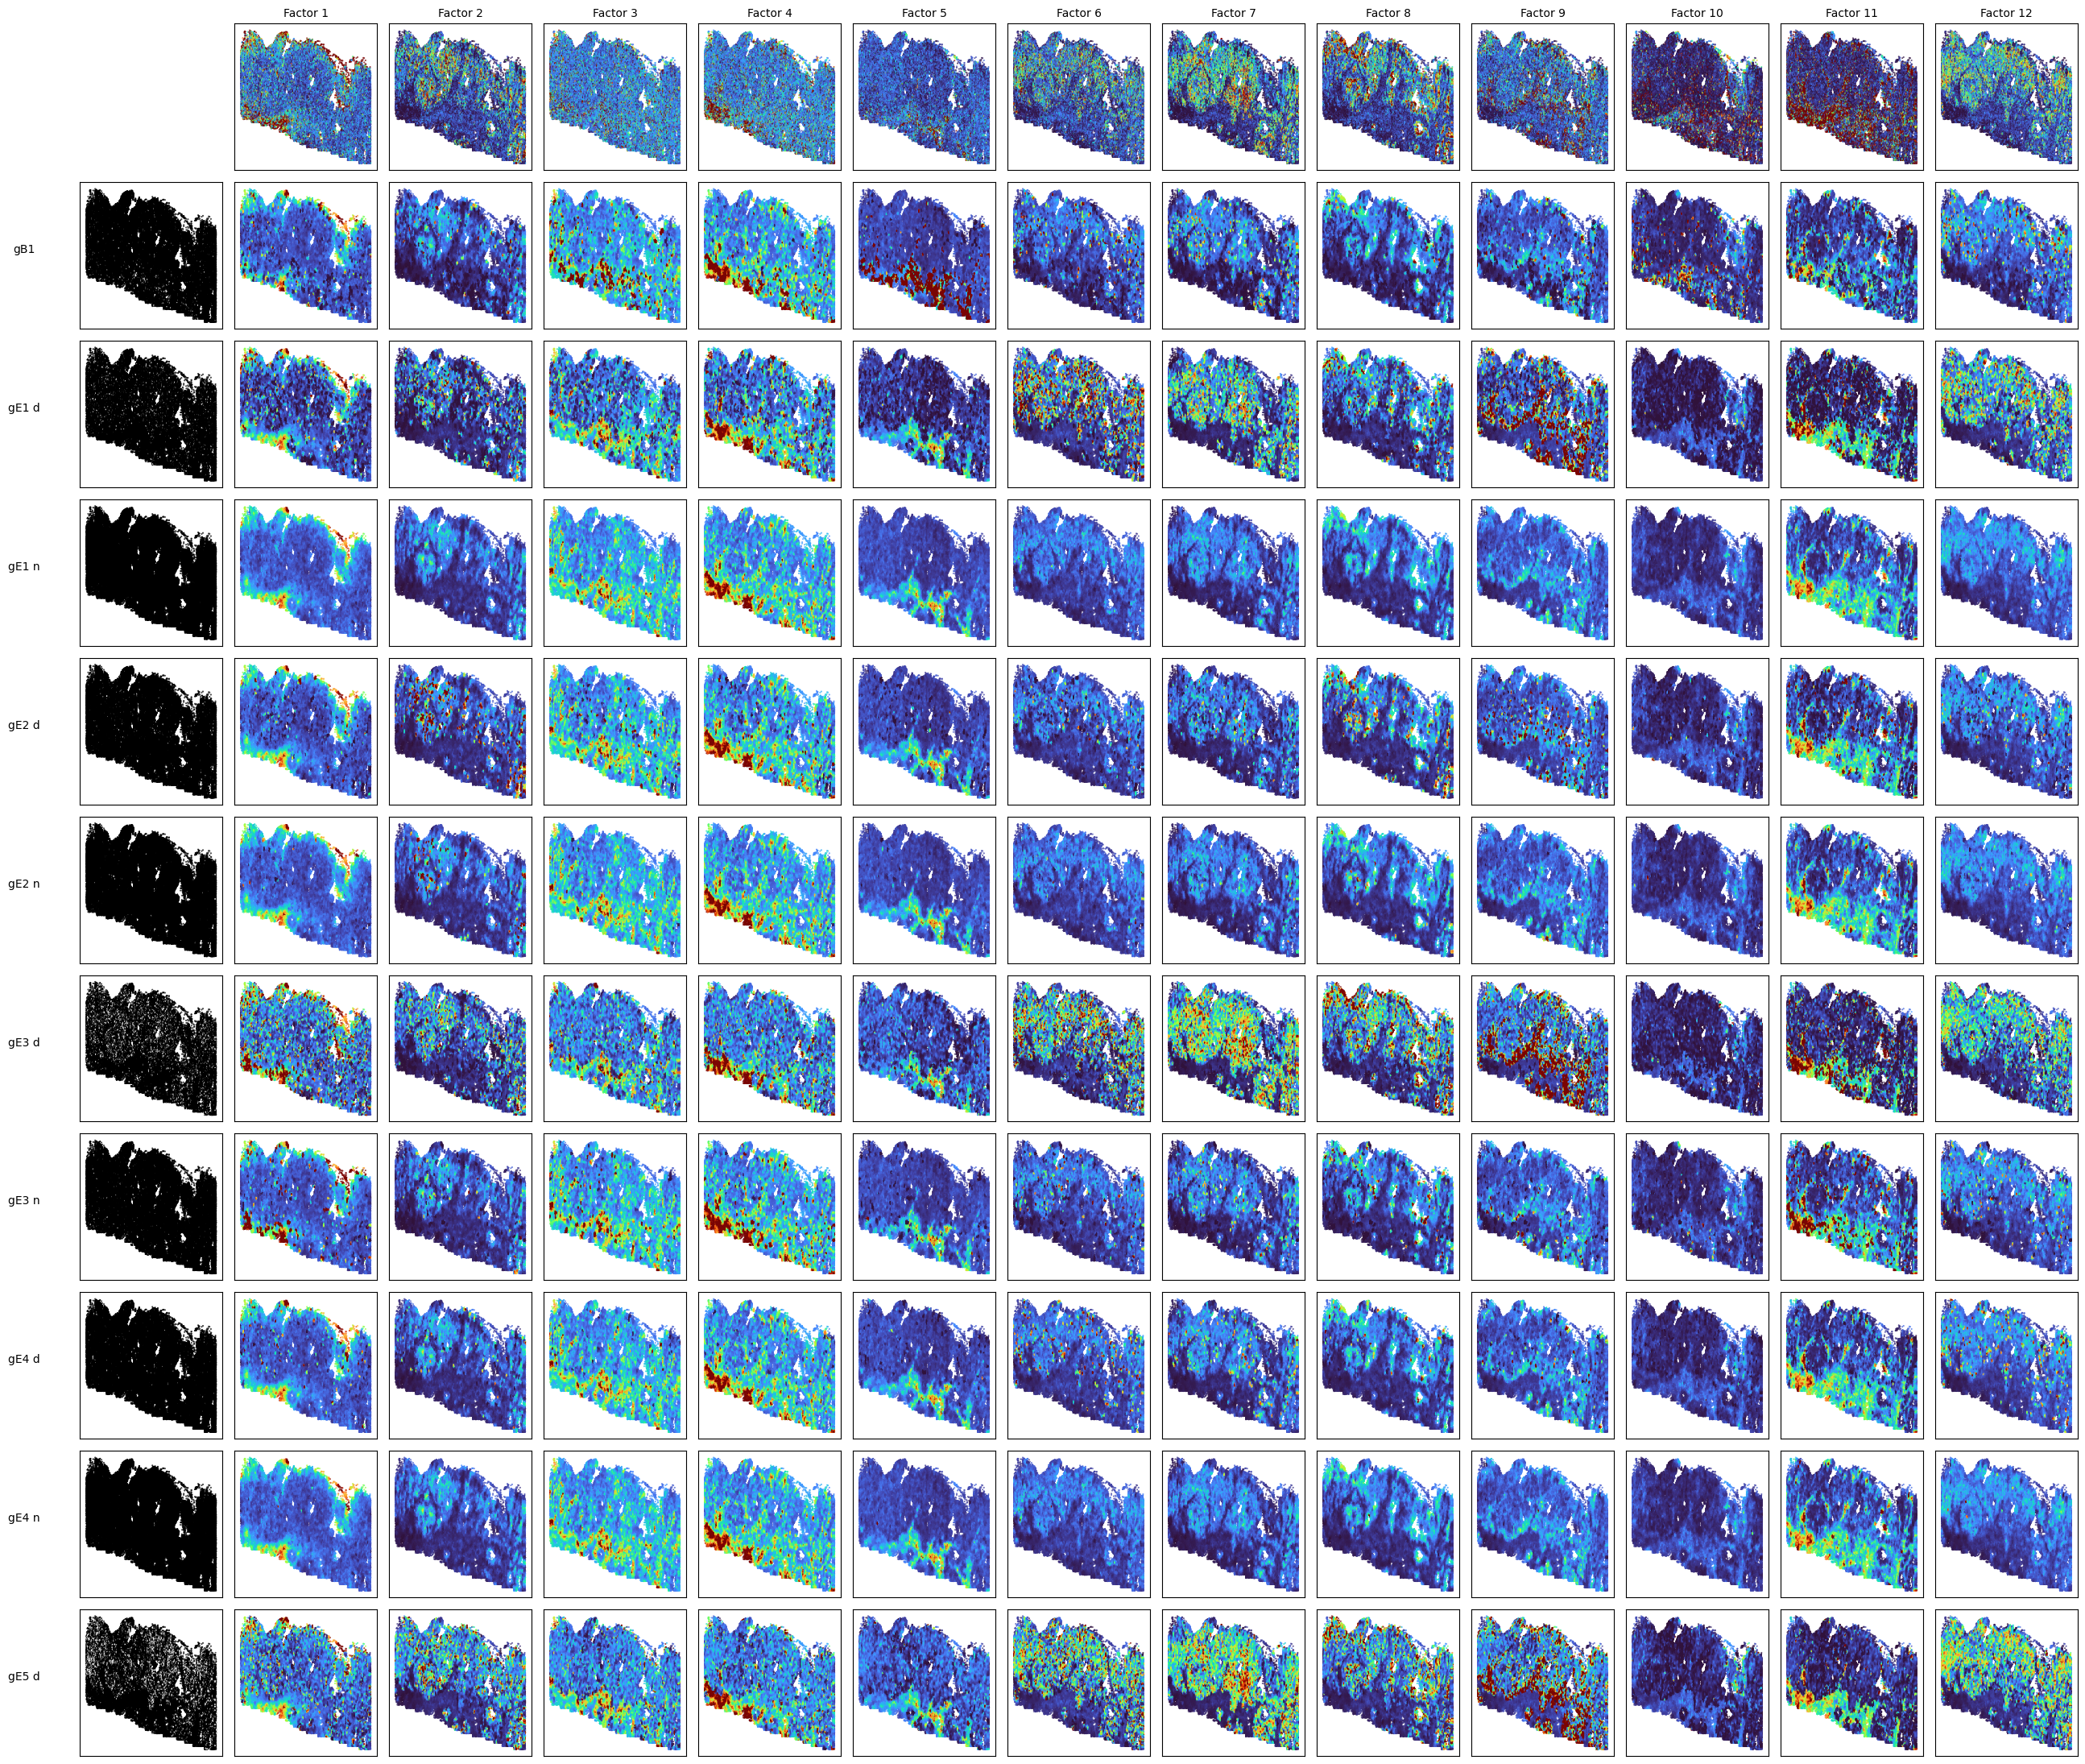
\includegraphics[width=0.98\linewidth]{MGGP_NSF_paper/HuColonCa-FFPE/posterior_1.png}
\caption{{\bf MERFISH CRC slices to show results from NSF versus MGNSF.}XXX }
\label{fig4a}
\end{figure}

\begin{figure}[!h]
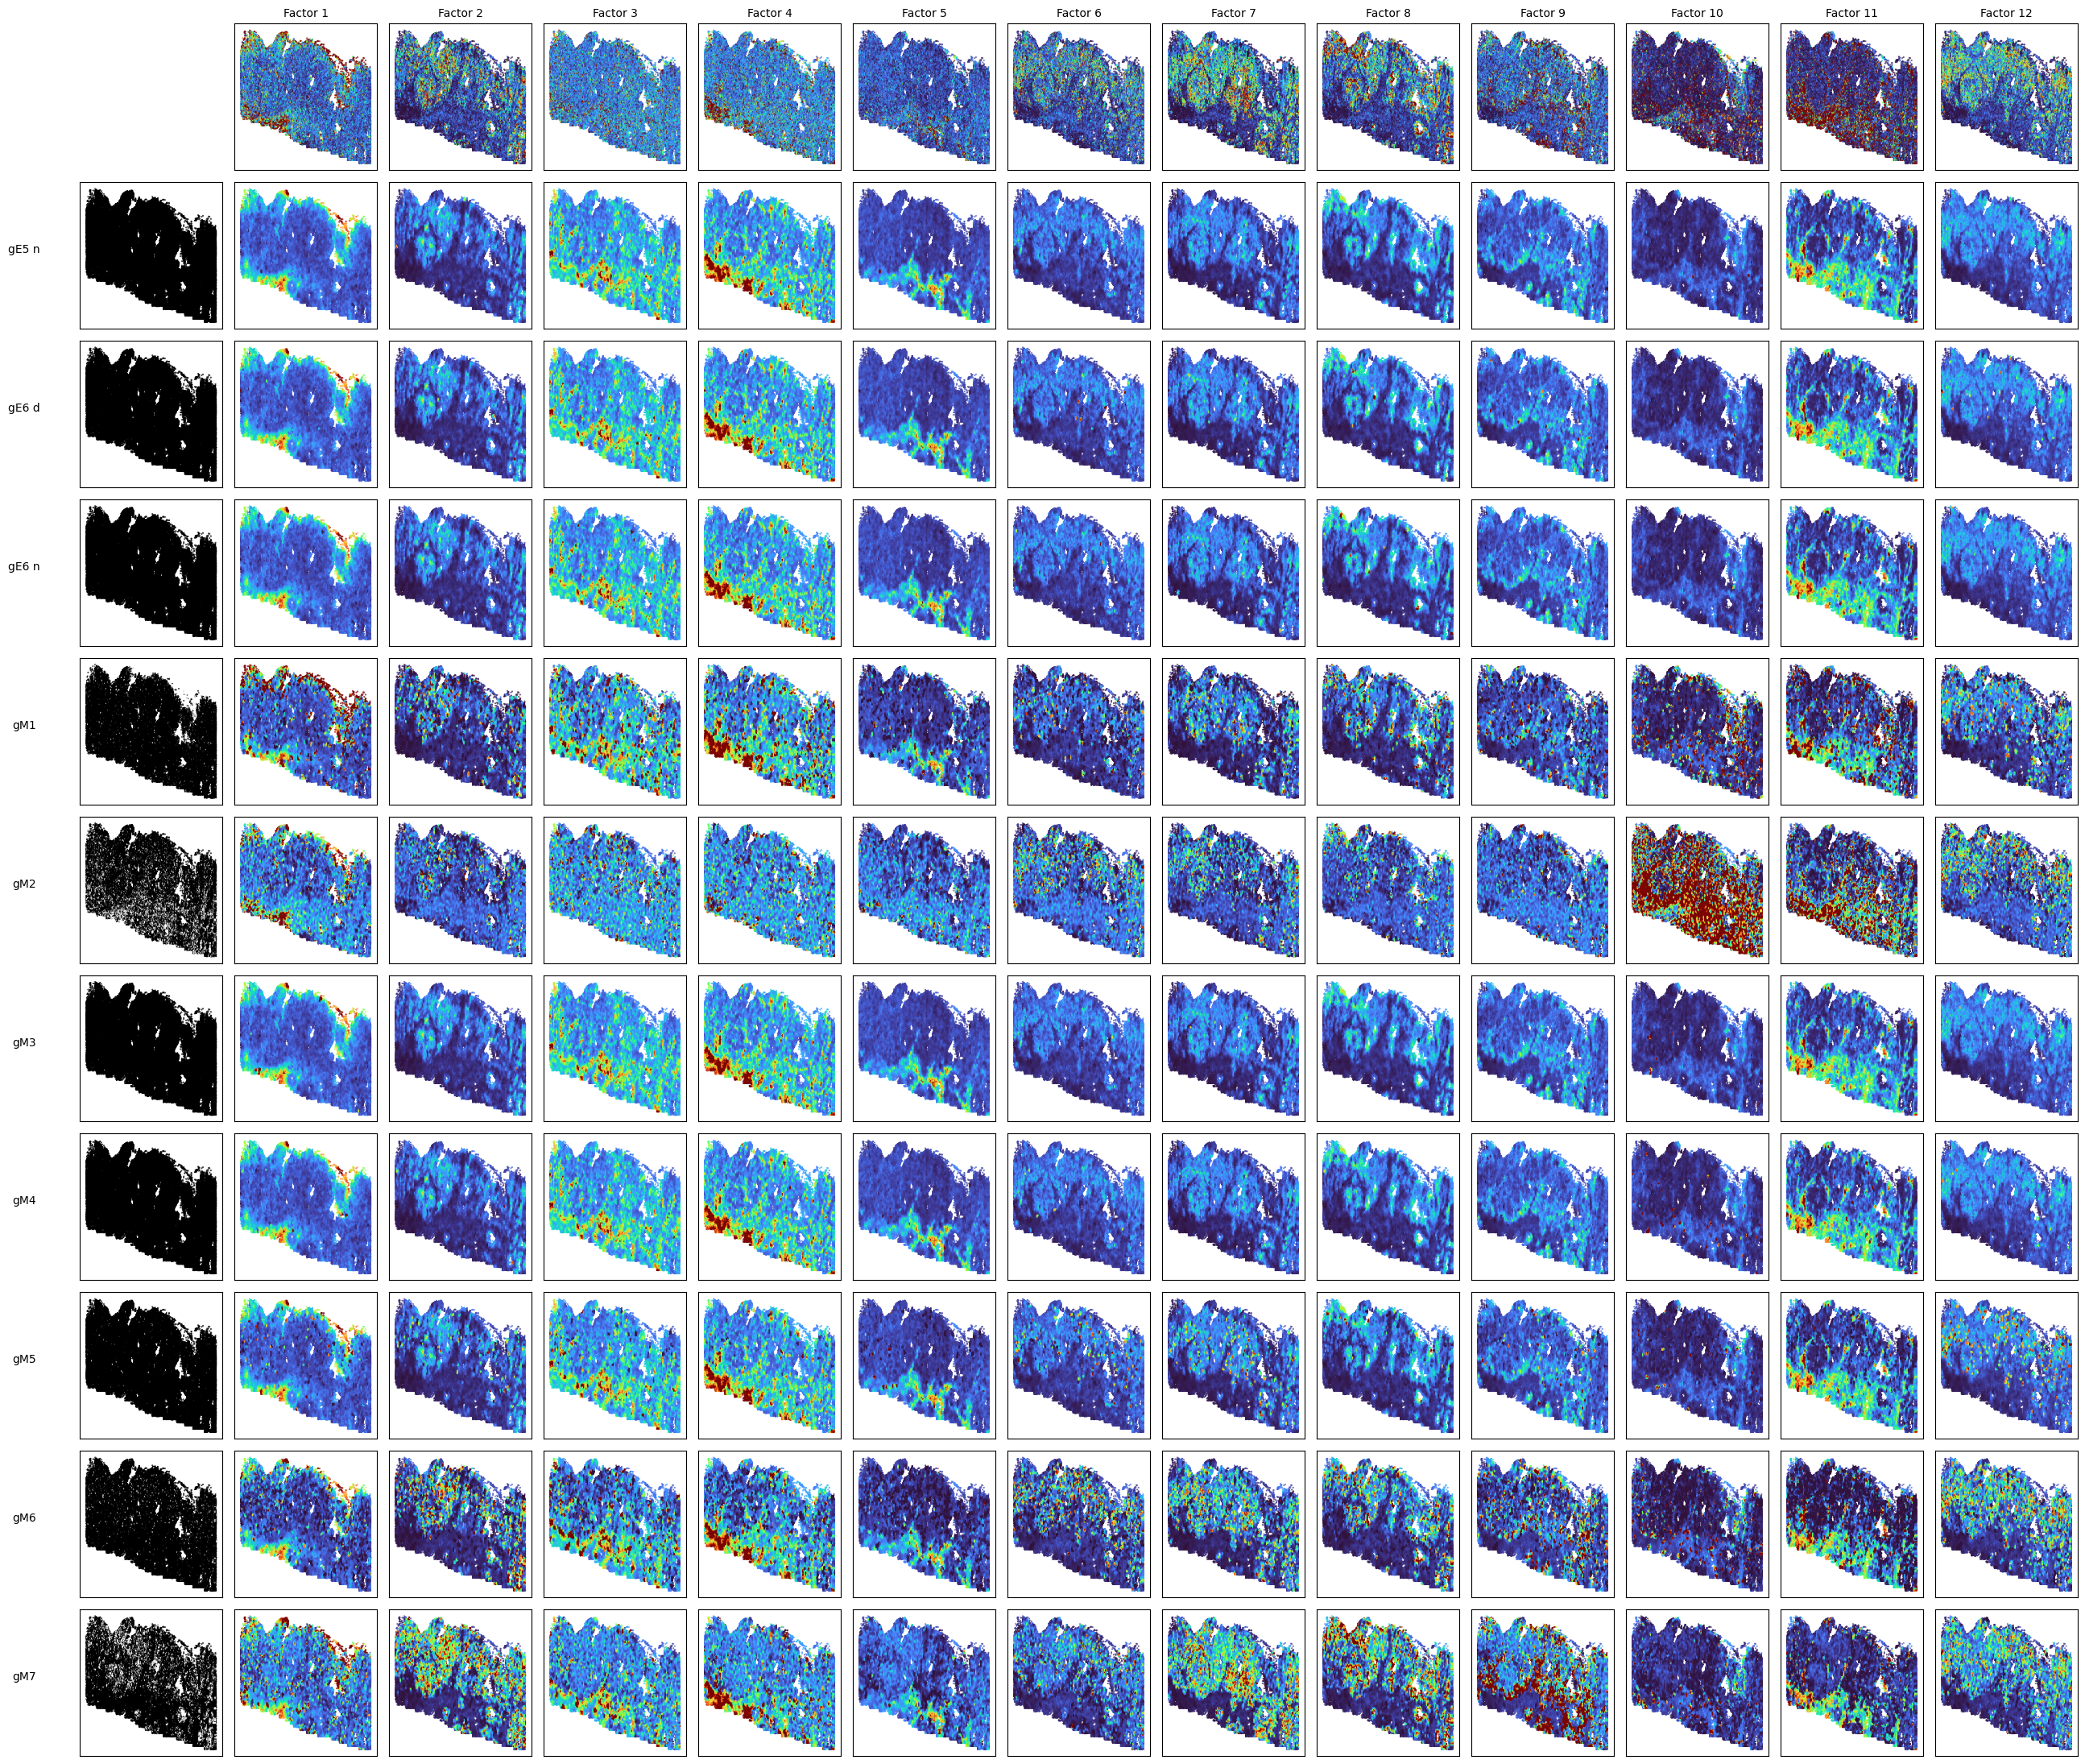
\includegraphics[width=0.98\linewidth]{MGGP_NSF_paper/HuColonCa-FFPE/posterior_2.png}
\caption{{\bf MERFISH CRC slices to show results from NSF versus MGNSF.}XXX }
\label{fig4b}
\end{figure}

\begin{figure}[!h]
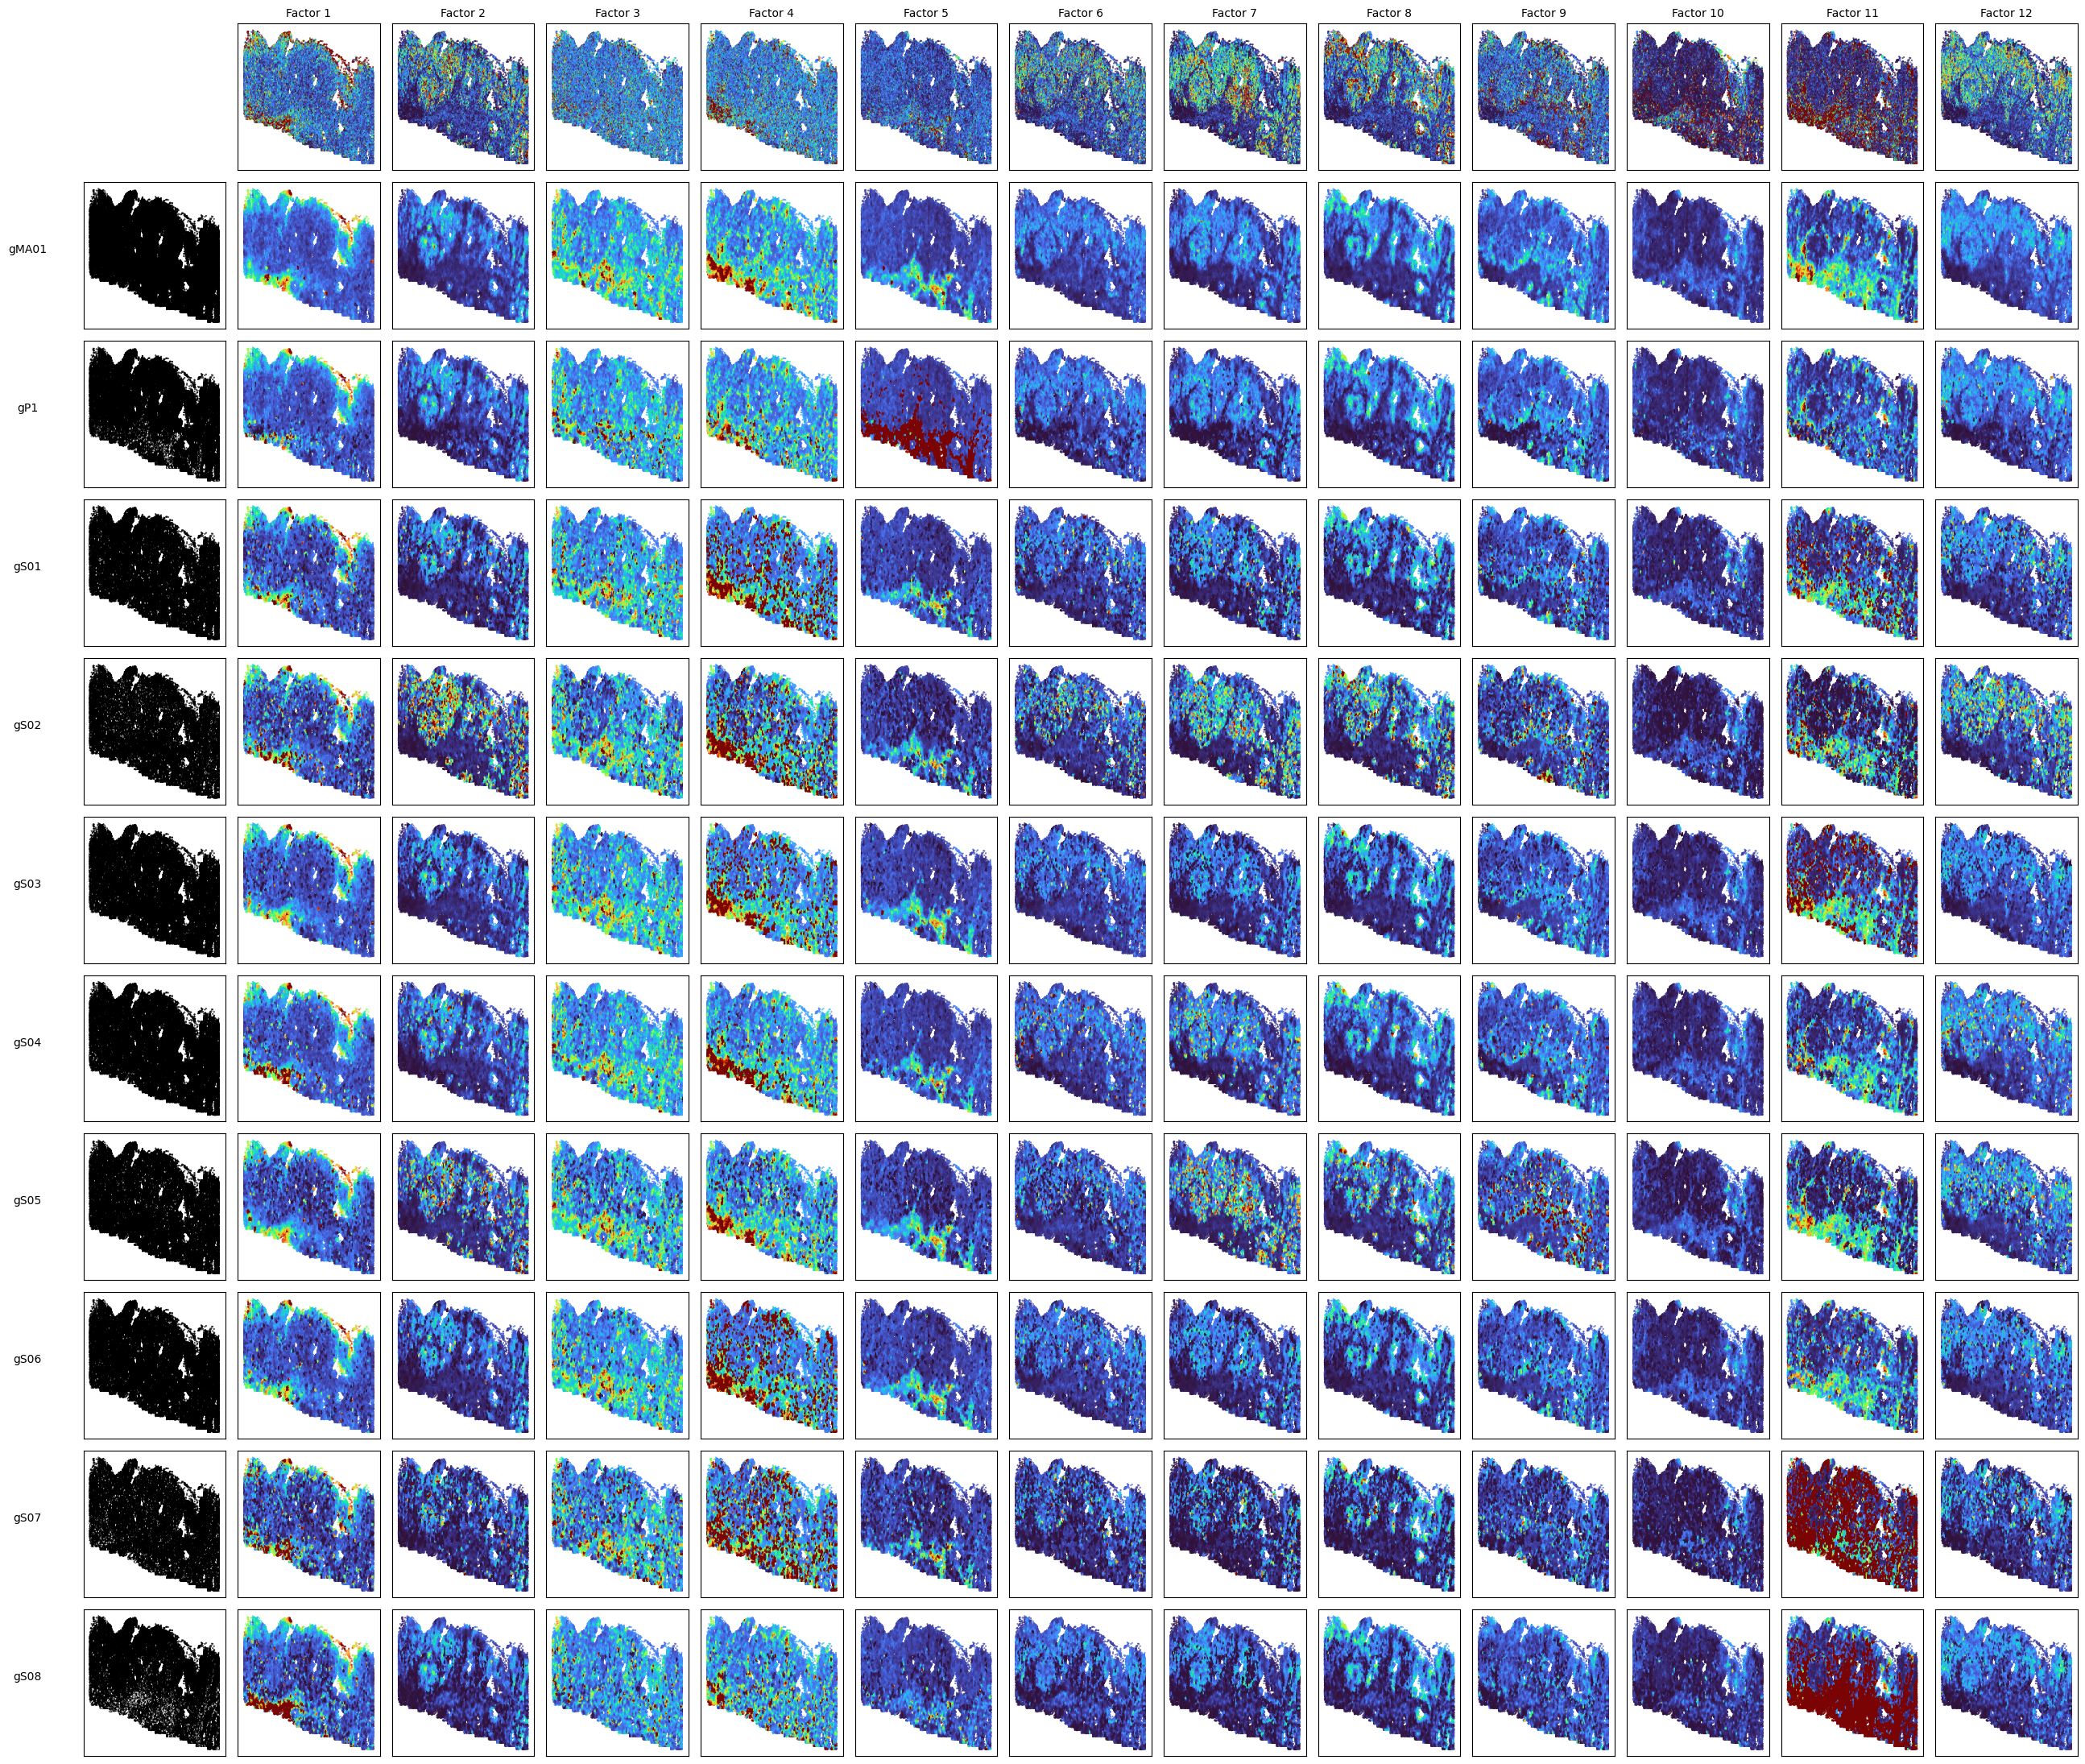
\includegraphics[width=0.98\linewidth]{MGGP_NSF_paper/HuColonCa-FFPE/posterior_3.png}
\caption{{\bf MERFISH CRC slices to show results from NSF versus MGNSF.}XXX }
\label{fig4c}
\end{figure}


\begin{figure}[!h]
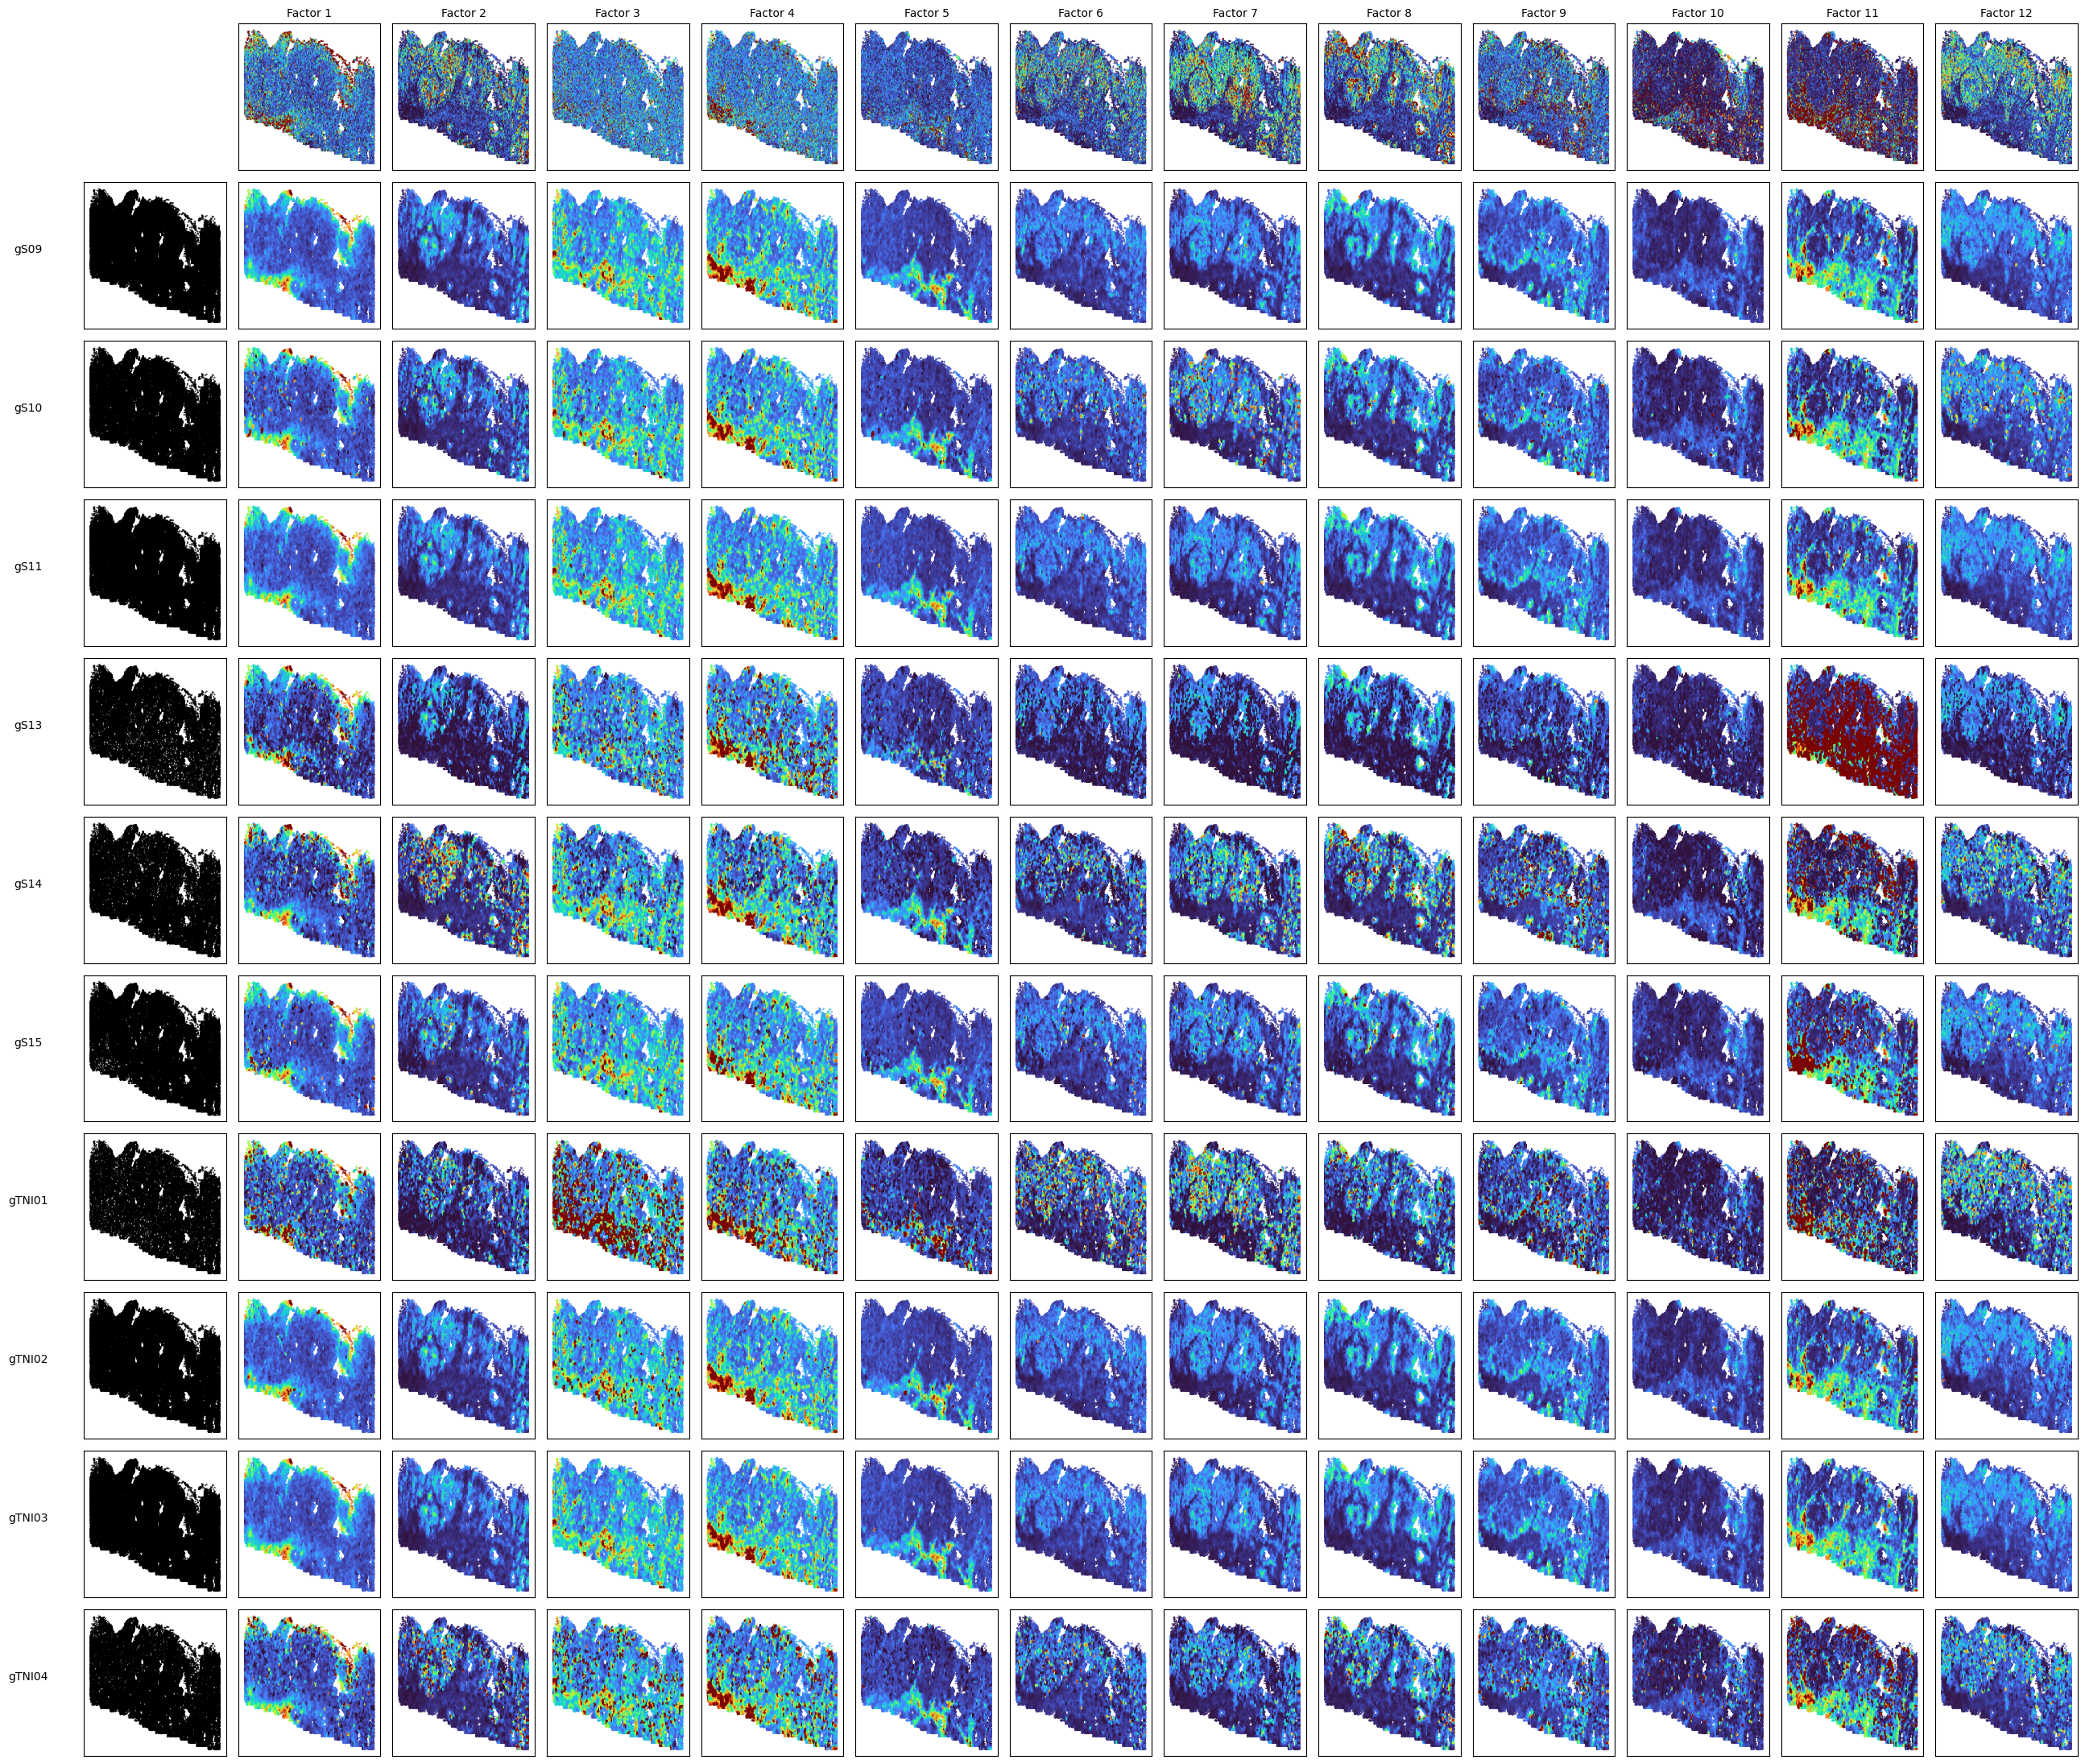
\includegraphics[width=0.98\linewidth]{MGGP_NSF_paper/HuColonCa-FFPE/posterior_4.png}
\caption{{\bf MERFISH CRC slices to show results from NSF versus MGNSF.}XXX }
\label{fig4d}
\end{figure}

\begin{figure}[!h]
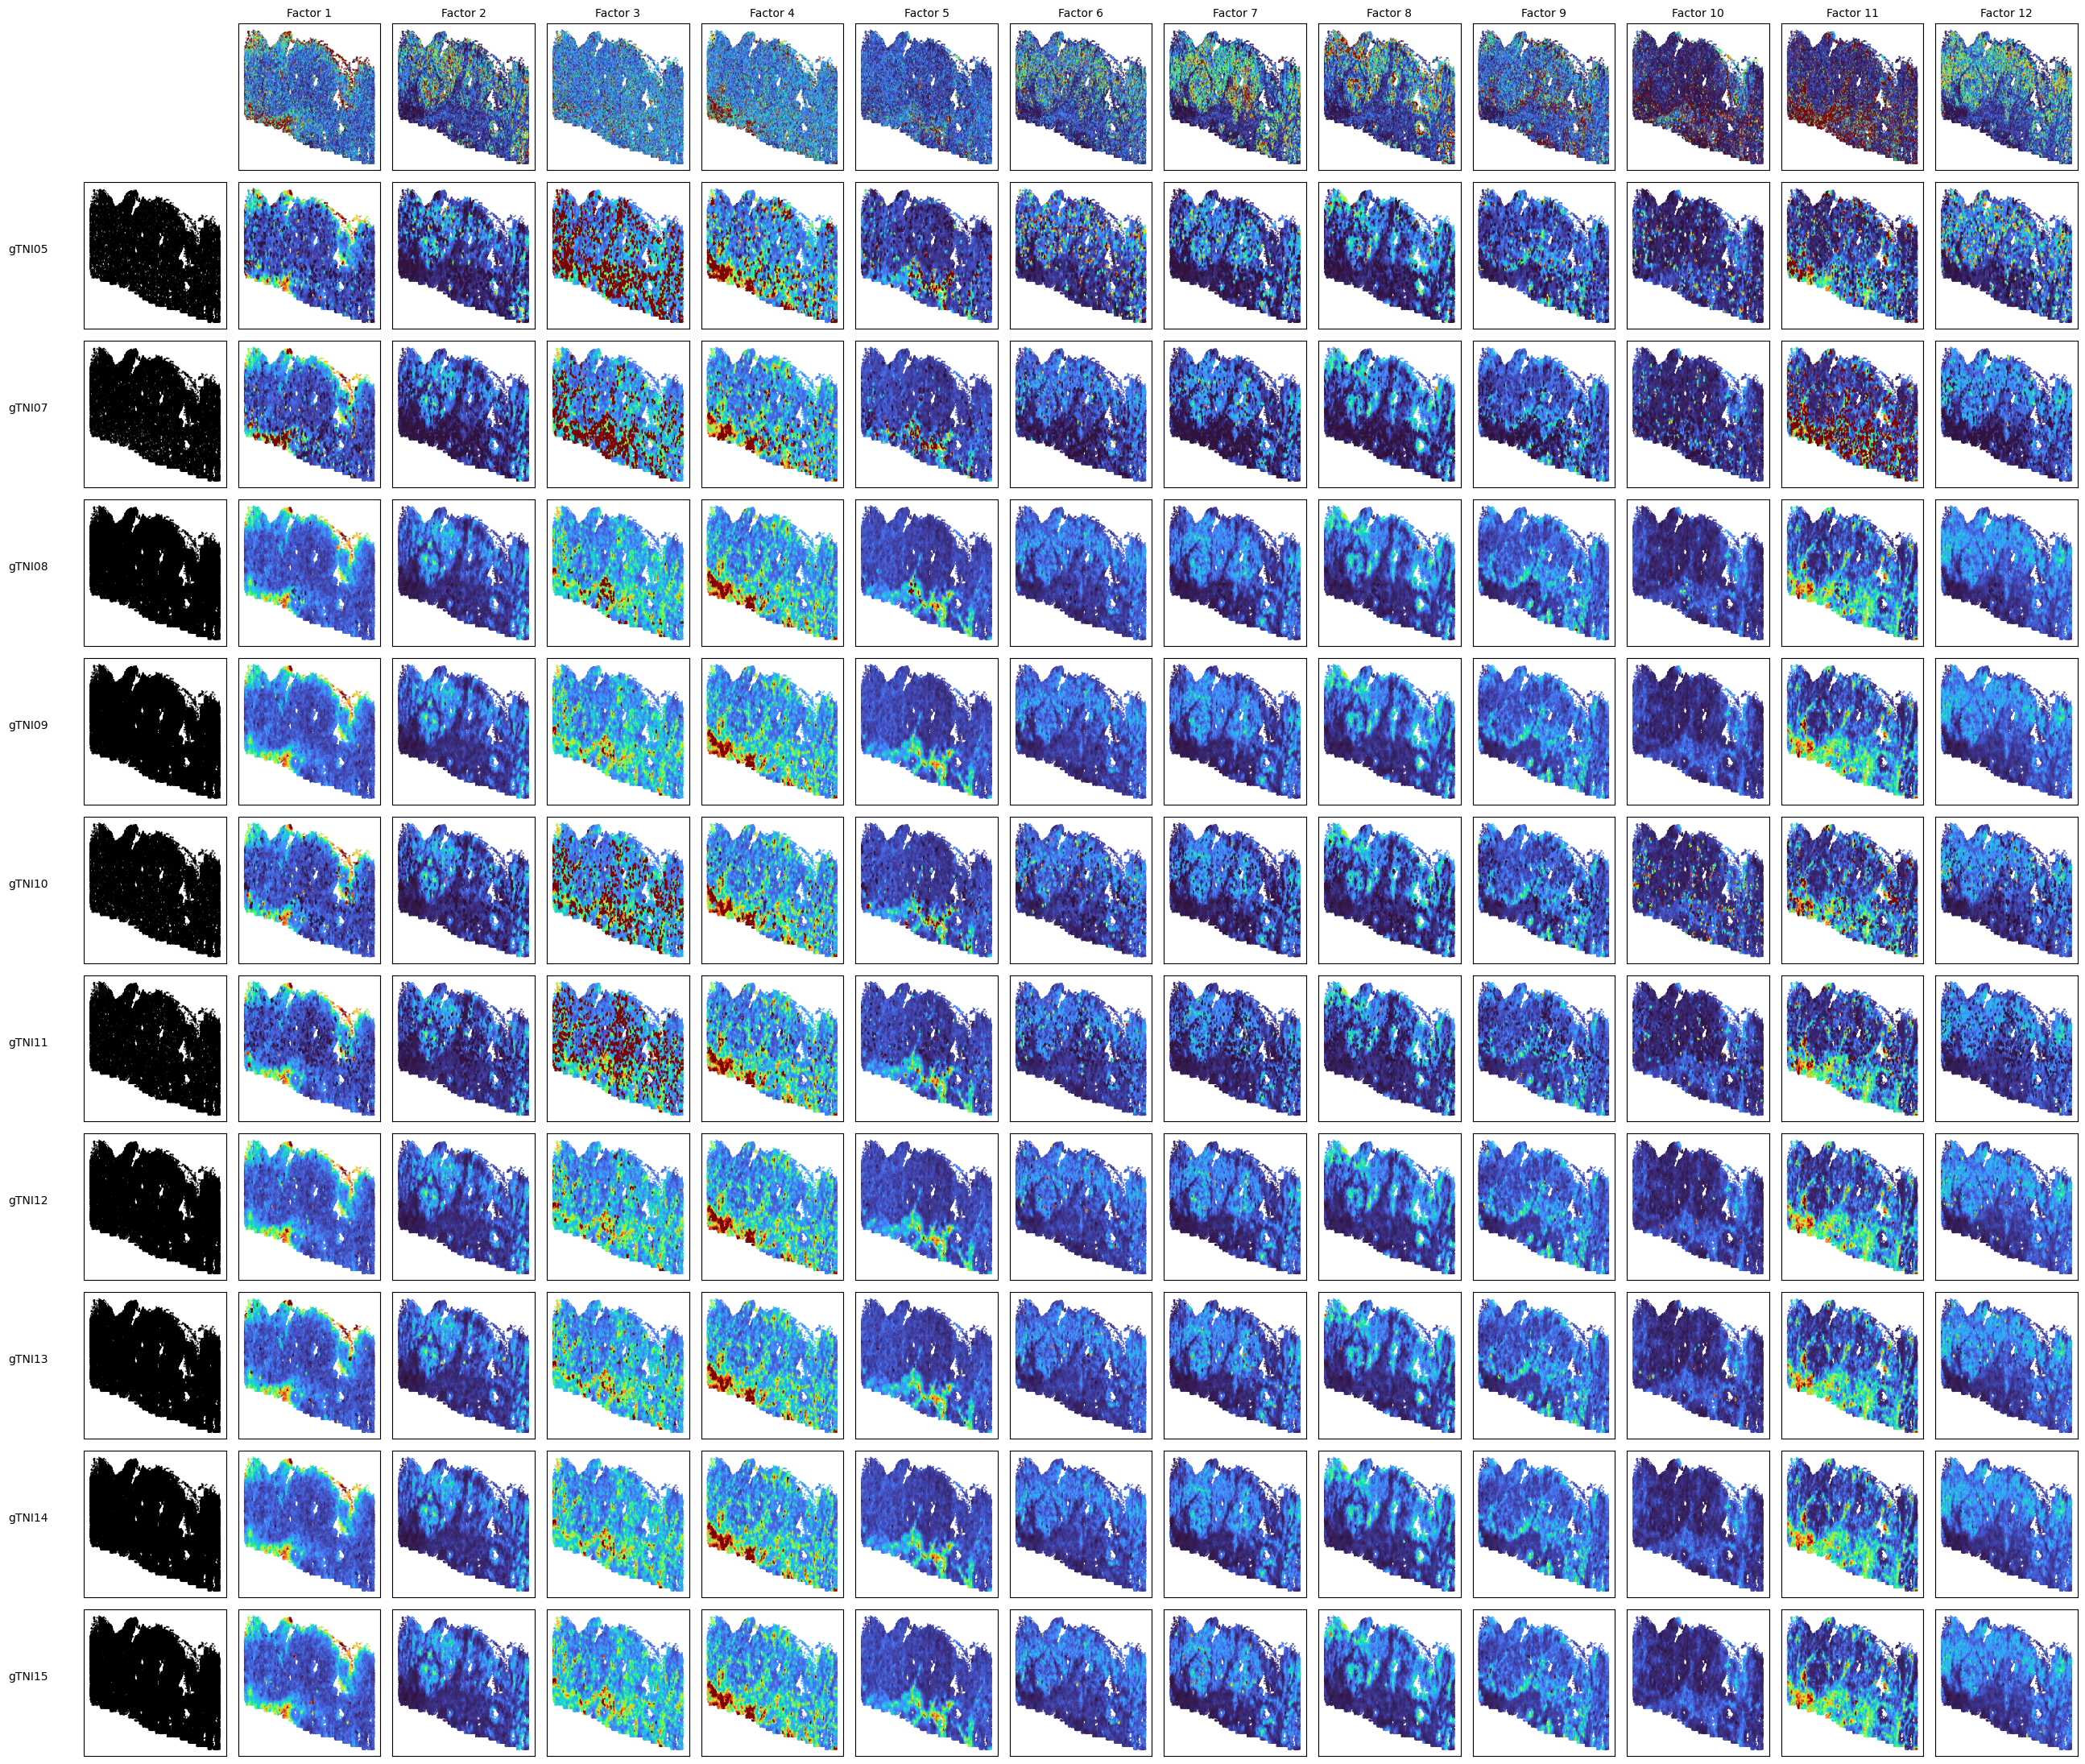
\includegraphics[width=0.98\linewidth]{MGGP_NSF_paper/HuColonCa-FFPE/posterior_5.png}
\caption{{\bf MERFISH CRC slices to show results from NSF versus MGNSF.}XXX }
\label{fig4e}
\end{figure}




% Fig 5: study of variance for MERFISH CRC slices
\begin{figure}[!h]
\includegraphics[width=0.98\linewidth]{}
\caption{{\bf MERFISH CRC slices to show variance estimates for MGNSF.}XXX }
\label{fig5-variance}
\end{figure}


% Fig 6: study of "conditional" gene expression differences for MERFISH CRC slices
\begin{figure}[!h]
\includegraphics[width=0.98\linewidth]{}
\caption{{\bf MERFISH CRC slices to show gene-specific reconstruction error for MGNSF.}XXX }
\label{fig6-gene-changes}
\end{figure}

% Fig 7: Liver healthy
\begin{figure}[!h]
\includegraphics[width=0.98\linewidth]{MGGP_NSF_paper/liver_fibrosis/factors.png}
\caption{{\bf MERFISH liver slices to show factors learned by the the VNNGP MGGP NSF} }
\label{fig7-liver}
\end{figure}


% Fig 8: Liver healthy conditionals
\begin{figure}[!h]
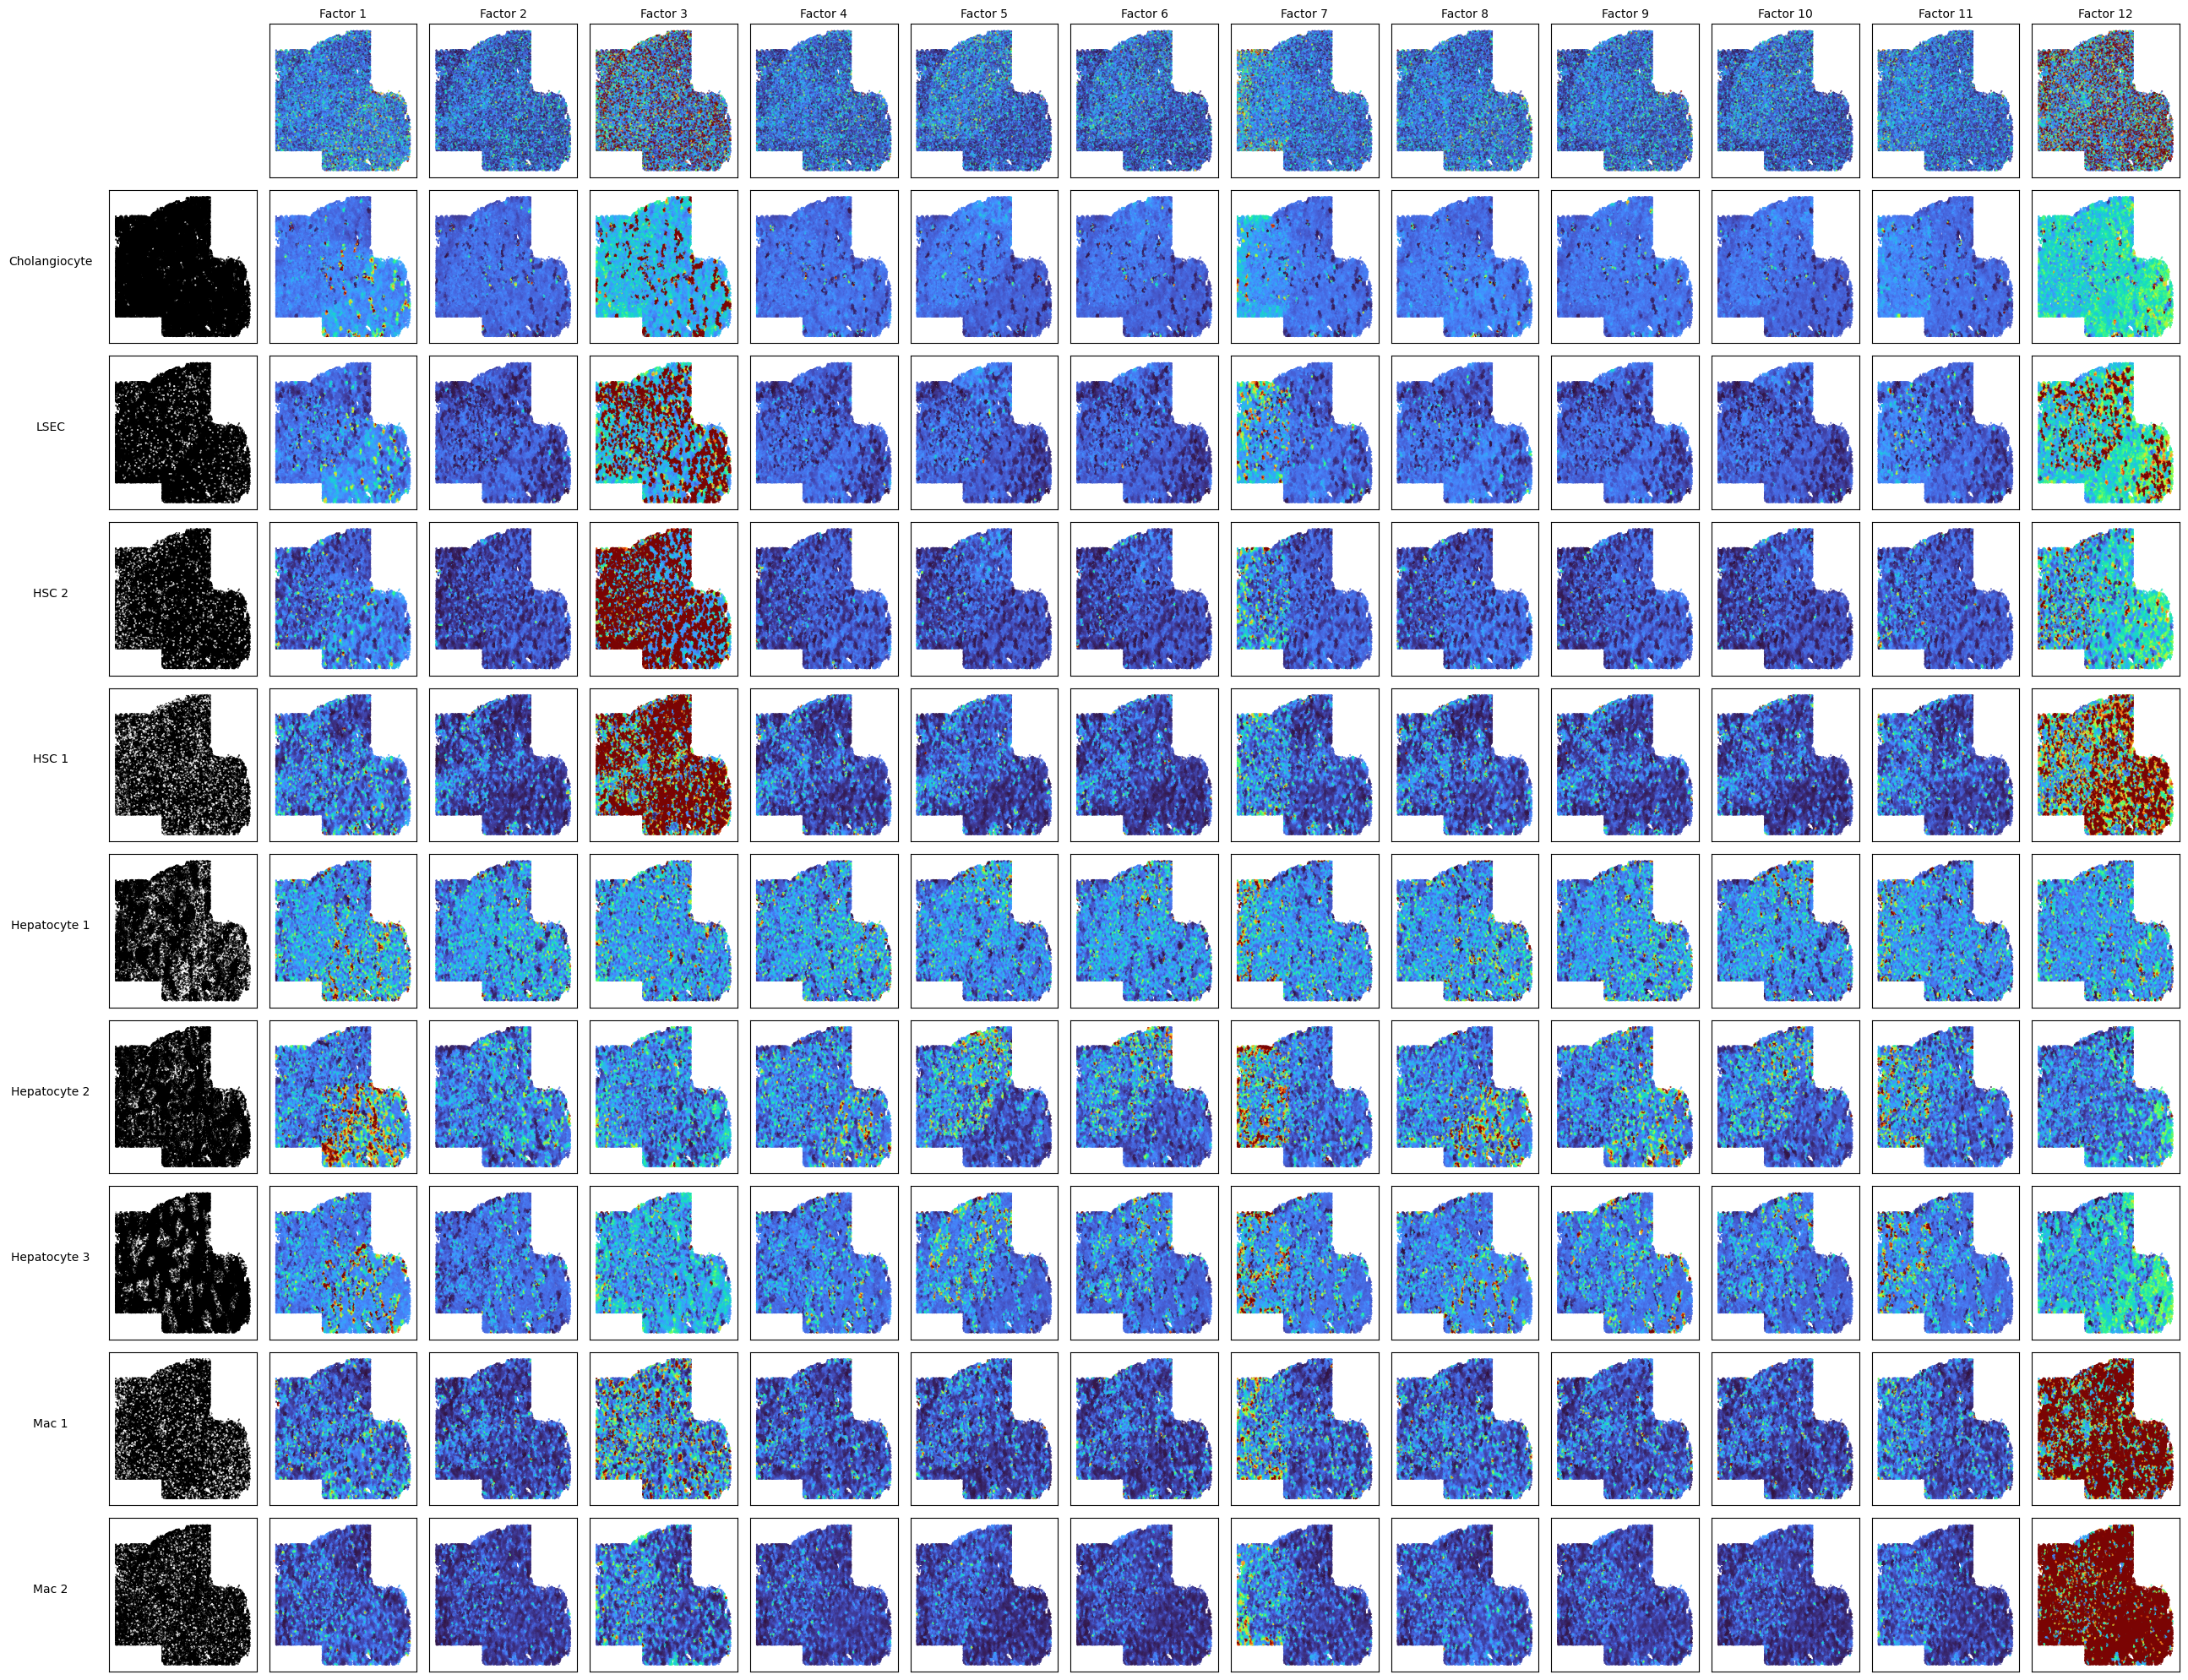
\includegraphics[width=0.98\linewidth]{MGGP_NSF_paper/liver_fibrosis/posteriors.png}
\caption{{\bf predictive conditional posteriors of MERFISH liver slices} }
\label{fig8-liver-posteriors}
\end{figure}


% Supplemental, mostly figures from vnngp, toy data experiments
\begin{figure}[!h]
\includegraphics[width=0.98\linewidth]{}


\caption{{\bf Visium brain slices to show factors, conditional factors, variance estimates, and gene specific changes for cell types using MGNSF.}XXX }
\label{figS1}
\end{figure}

\clearpage
\section*{Materials and methods}

\subsection*{ Multigroup Nonnegative Spatial Factorization (MNSF)}

Multigroup Nonnegative Spatial Factorization (MNSF) expands NSF to incorporate both spatial and cell-type information through multigroup Gaussian processes (MGGPs)\cite{Li2021-fv}. The model takes as input: a spatial transcriptomics count matrix \( Y \in \mathbb{R}^{N \times J} \), spatial coordinates \( X \in \mathbb{R}^{N \times D} \), and group labels \( C = \{c_1, c_2, \ldots, c_N\} \) (e.g., cell types or clusters).

The model is:
\begin{align*}
y_{ij} &\sim \text{Poisson}(\nu_i \lambda_{ij}) \\
\lambda_{ij} &= \sum_{l=1}^L w_{jl} \exp(f_{il}) \\
f_{il} &\sim \text{MGGP}\left(0, K_l\left((x_i, c_i), (X, C)\right)\right)
\end{align*}

Here, \( \nu_i \) is a per-spot normalization term, \( w_{jl} \) are gene loadings constrained to be nonnegative (via softplus transformation), and \( f_{il} \) are spatial latent factors with a multigroup Gaussian process prior. The covariance function is defined over both space and group label:

\begin{align*}
K\left((x, c), (x', c')\right) = \sigma^2 \left(\alpha^2 d_{cc'}^2 + 1\right)^{-D/2} \exp\left( -\frac{\beta^2 \|x - x'\|^2}{\alpha^2 d_{cc'}^2 + 1} \right)
\end{align*}

where \( d_{cc'} \) is a group-level distance (e.g., discrete or hierarchical), and \( \alpha \), \( \beta \), and \( \sigma \) are kernel hyperparameters. This formulation enables smooth signal sharing across related cell types while allowing for structured differences in spatial expression patterns.

\vspace{1em}

\subsection*{ Hybrid Spatial–Nonspatial Model for Denoising}

To improve robustness, we extend MNSF into a hybrid model that captures both spatial and nonspatial structure. In this formulation, each latent dimension is split into a spatial component \( f_{il} \) and a nonspatial component \( h_{il} \), yielding:

\begin{align*}
y_{ij} &\sim \text{Poisson}(\nu_i \lambda_{ij}) \\
\lambda_{ij} &= \sum_{l=1}^L w_{jl} \exp(f_{il}) + \sum_{l=1}^L v_{jl} \exp(h_{il}) \\
f_{il} &\sim \text{MGGP}\left(0, K_l\left((x_i, c_i), (X, C)\right)\right) \\
h_{il} &\sim \mathcal{N}(0, s_l^2)
\end{align*}

The gene loadings \( w_{jl} \) and \( v_{jl} \) are nonnegative and control the contribution of spatial and nonspatial latent factors, respectively. The spatial factors \( f_{il} \) capture coherent gene expression structure that varies over space and group, while the \( h_{il} \) terms absorb residual variation that is not spatially structured. This decomposition acts as a denoising mechanism, preventing the model from fitting noise or local artifacts as spatial signal. Spatial factors tend to converge to smooth patterns capturing dominant tissue-scale variation (see Fig.~1).

The model is initialized using nonnegative matrix factorization (NMF), which accelerates convergence and stabilizes training. Variational inference with sparse inducing points is used for scalability, and softplus transformations are applied to all constrained parameters to improve numerical stability.


\subsection*{Cell-type Conditional Posterior Experiments}

To understand the extent to which spatial patterns in MNSF are influenced by cell-type labels, we conducted a series of \textit{in silico} perturbation experiments. Specifically, we modified the cell-type labels \( C \) used as inputs to the multigroup Gaussian process kernel and recomputed the posterior predictive distribution of the spatial factors \( F \) under the new labels. This enables us to measure the conditional dependence of each spatial factor on the cell-type context.

At training time, the posterior predictive distribution is given by:
\[
q(F \mid X, C_X) = \int p(F \mid U, X, C_X, Z, C_Z) \, q(U) \, dU,
\]
where \( q(U) \) is the variational distribution over inducing variables, and \( F \sim q(F \mid X, C_X) \) is sampled to construct the Poisson rate used in the likelihood.

During the \textit{in silico} perturbation experiments, we keep the spatial coordinates \( X \) fixed but modify the label inputs \( C_X \) to a new configuration \( C_X^{\text{new}} \). We then sample from the recomputed posterior:
\[
F^{\text{new}} \sim q(F \mid X, C_X^{\text{new}}),
\]
allowing us to observe how predicted spatial factors change under altered label assignments.

For each spatial factor \( f_l \), we selected a fixed spatial coordinate \( x_i \) and replaced its original cell-type label \( c_i \) with a different label \( c_i' \), while keeping all other inputs unchanged. We then recomputed the predictive posterior \( q(f_{il} \mid x_i, c_i') \) using the variational inference framework described in Supplemental Section~\ref{sec4}. If the spatial factor \( f_l \) exhibits strong cell-type specificity, its posterior mean or variance should change significantly under this perturbation.

We performed these experiments across multiple datasets and visualized the resulting spatial patterns after setting all cell-type labels to a single target type. This yielded a controlled view of how spatial factors behave when conditioned on different cell-type contexts. In MERFISH FFPE Colon (Figure \ref{fig4a}), we observed several factors whose intensity patterns were strongly modulated by the input label, suggesting that those factors encode cell-type-specific spatial structure. In contrast, other factors remained largely unchanged, indicating they capture spatial programs shared across cell types.

These conditional posterior analyses reveal that MNSF can disentangle spatial variation that is tightly coupled to cellular identity from variation that is broadly shared. By manipulating cell-type labels independently of spatial coordinates, MNSF supports a novel form of exploratory analysis that is not available in standard GP-based spatial models. This framework provides a promising foundation for future work in virtual perturbation, tissue engineering simulations, and hypothesis generation regarding spatial gene regulation.



\subsection*{ Variational Nearest Neighbor Model}

To improve scalability while maintaining the ability to model cell-type-specific spatial variation, we replace the full multigroup Gaussian process (MGGP) prior with a variational nearest neighbor Gaussian process (VNNGP) prior. This formulation significantly reduces computational overhead by conditioning each latent function value \( f_{il} \) on a small set of neighboring inducing points.

The MNSF model under the VNNGP approximation is defined as:
\begin{align*}
y_{ij} &\sim \text{Poisson}(\nu_i \lambda_{ij}) \\
\lambda_{ij} &= \sum_{l=1}^L w_{jl} \exp(f_{il}) \\
f_{il} &\sim \text{VNNGP}\left(0, K_l\left((x_i, c_i), \{(z_k, c_k)\}_{k \in \mathcal{N}(i)}\right)\right) 
\end{align*}

Here, \( \mathcal{N}(i) \) denotes the index set of the \( K \) nearest inducing points to \( (x_i, c_i) \) under a joint spatial and label-aware distance metric. Instead of conditioning on all inducing points as in standard MGGPs, each spatial factor \( f_{il} \) is now modeled as a GP conditioned only on a local subset of \( K \) points, yielding substantial savings in time and memory.

The VNNGP approximation reduces the computational complexity of inference from \( \mathcal{O}(LNM^2) \) to \( \mathcal{O}(LNK^2) \), where \( N \) is the number of spatial locations, \( M \) is the total number of inducing points, and \( K \ll M \) is the number of nearest neighbors used per observation. This makes the model well suited for large-scale spatial transcriptomics datasets, including those with hundreds of thousands of spots.

During variational inference, the inducing variables are shared across the entire tissue but grouped by label during neighbor selection, allowing both global sharing and local adaptation of spatial structure. Unlike in the regular variational MGGP case, we don't apply whitening transformations, but instead, we derived a KL-divergence approximation (see methods) of a multivariate normal variational inducing distribution to keep cell-to-cell relationships but also enforce a proper GP prior on the factors.

This nearest neighbor-based approximation enables MNSF to scale to large spatial transcriptomics datasets without compromising the model’s ability to recover cell-type-aware spatial factors.

One limitation of the cell-type conditional posterior experiments described in Section~2.3 is their reliance on a relatively small number of inducing points. For instance, using 5{,}000 inducing points to represent a dataset with over one million spatial locations introduces a resolution gap that limits the model’s ability to generalize across cell-type perturbations. In such regimes, full-posterior updates under perturbed cell-type labels may fail to capture localized structure, especially when the spatial resolution of inducing points is relative to the density of the data. The VNNGP framework helps address this limitation by conditioning each prediction on a local neighborhood of inducing points, improving spatial fidelity and robustness to label-specific variation in large-scale experiments.






\begin{table}[!ht]
\begin{adjustwidth}{-2.25in}{0in} % Comment out/remove adjustwidth if table fits in text column.
\centering
\caption{
{\bf Comparison of spatial transcriptomics methods.} Methods differ in whether they incorporate spatial information, account for cell types, use nonnegativity constraints, and in their modeling goals.}
\begin{tabular}{|l|c|c|c|l|l|}
\hline
\textbf{Method} & \textbf{Spatial} & \textbf{Cell-Type} & \textbf{Nonneg.} & \textbf{Inputs} & \textbf{Goal} \\ \thickhline
PCA / FA         & No  & No  & No  & Expression only & Linear projection \\
NMF / PNMF       & No  & No  & Yes & Expression only & Parts-based decomposition \\
SpatialPCA       & Yes & No  & No  & Expression + spatial & Spatial smoothing of latent space \\
NSF              & Yes & No  & Yes & Expression + spatial & Interpretable spatial decompositions \\
MEFISTO          & Yes & No  & No  & Expression + spatial & Continuous time/space variation \\
SpaTopic         & Yes & No  & Yes & Expression + graph & Domain discovery \\
FISHFactor       & Yes & No  & Yes & smFISH coords & Subcellular modeling \\
C-SIDE           & No  & Yes & Optional & Expression + covariates & Expression variation from metadata \\
cell2location    & Yes & Yes & No  & ST + scRNA-seq & Spatial deconvolution \\
DistMap          & Yes & No  & No  & scRNA-seq + spatial atlas & Map cells to embryo \\
Starfysh         & Yes & No  & No  & Expression + graph & Graph convolutional smoothing \\
stKeep           & Yes & No  & No  & Expression + kNN graph & Region segmentation \\
MNSF (Ours)      & Yes & Yes & Yes & Expression + spatial + cell-type &  Spatial+cell-type decompositions\\
\hline
\end{tabular}

\label{table:method-comparison}
\end{adjustwidth}
\end{table}

\clearpage

\subsection*{Full KL Divergence for VNNGP}

We approximate the KL divergence between the variational distribution \( q(U) \) and the GP prior \( p(U) \) using a locally conditional chain rule factorization. Let \( U = [U_1, \dots, U_M] \) be the collection of inducing variables. The prior and variational distributions are factorized as:

\begin{align*}
p(U) &= p(U_1) \prod_{j=2}^{M} p(U_j | U_{1, \dots, j-1}) \approx \prod_{j=1}^{M} p(U_j | U_{n(j)}) \\
q(U) &= q(U_1) \prod_{j=2}^{M} q(U_j | U_{1, \dots, j-1}) \approx \prod_{j=1}^{M} q(U_j | U_{n(j)})
\end{align*}

This approximation allows us to express the KL divergence as a sum of local terms:


\begin{align*}
\mathrm{KL}(q(U) \| p(U)) 
&= \mathbb{E}_{q(U)} \left[ \log \frac{q(U)}{p(U)} \right] \\
&\approx \sum_{j=1}^{M} \mathbb{E}_{q(U)} \left[ \log \frac{q(U_j | U_{n(j)})}{p(U_j | U_{n(j)})} \right] \\
&= \sum_{j=1}^{M} \mathbb{E}_{q(U_{n(j)})} \left[ \mathbb{E}_{q(U_j | U_{n(j)})} \left[ \log \frac{q(U_j | U_{n(j)})}{p(U_j | U_{n(j)})} \right] \right]\\
&= \sum_{j=1}^{M} \mathbb{E}_{q(U_{n(j)})} \left[ \mathrm{KL}(q(U_j | U_{n(j)}) \| p(U_j | U_{n(j)})) \right]
\end{align*}


Each term in the sum compares the conditional posterior and prior distributions. These are Gaussian conditionals:

\begin{align*}
p(U_j | U_{n(j)}) &= \mathcal{N}\left( \beta_j^\top U_{n(j)}, \; \tau_j^2 \right) \\
q(U_j | U_{n(j)}) &= \mathcal{N}\left( m_j + \alpha_j^\top (U_{n(j)} - m_{n(j)}), \; \tilde{\tau}_j^2 \right)
\end{align*}

Where:

\begin{align*}
\beta_j^\top &= K_{jn(j)} K_{n(j)n(j)}^{-1}, \quad
\tau_j^2 = k_{jj} - K_{jn(j)} K_{n(j)n(j)}^{-1} K_{n(j)j} \\
\alpha_j^\top &= S_{jn(j)} S_{n(j)n(j)}^{-1}, \quad
\tilde{\tau}_j^2 = s_{jj} - S_{jn(j)} S_{n(j)n(j)}^{-1} S_{n(j)j}
\end{align*}

The KL divergence between two univariate Gaussians is:

\[
\mathrm{KL}(q \| p) = \frac{1}{2} \left[ \log \frac{\tau_j^2}{\tilde{\tau}_j^2} 
+ \frac{\tilde{\tau}_j^2}{\tau_j^2} 
+ \frac{\mathbb{E}_{q(U_{n(j)})}\left[(\mu_q - \mu_p)^2\right]}{\tau_j^2} - 1 \right]
\]

To evaluate the expectation term \( \mathbb{E}_{q(U_{n(j)})}[(\mu_q - \mu_p)^2] \), we write:

\[
\mu_q - \mu_p = m_j + \alpha_j^\top (U_{n(j)} - m_{n(j)}) - \beta_j^\top U_{n(j)} 
= (\alpha_j - \beta_j)^\top U_{n(j)} + (m_j - \alpha_j^\top m_{n(j)})
\]

Then use the standard quadratic expectation identity for Gaussians:

\[
\mathbb{E}_{x \sim \mathcal{N}(\mu, \Sigma)}[(a^\top x + b)^2] = a^\top \Sigma a + (a^\top \mu + b)^2
\]

Applying this gives:

\[
\mathbb{E}_{q(U_{n(j)})}[(\mu_q - \mu_p)^2] = 
(\alpha_j - \beta_j)^\top S_{n(j)n(j)} (\alpha_j - \beta_j) + 
\left[(\alpha_j - \beta_j)^\top m_{n(j)} + (m_j - \alpha_j^\top m_{n(j)})\right]^2
\]

This expectation can be expanded further and simplified as:

\[
= \alpha_j^\top S_{n(j)n(j)} \alpha_j + \beta_j^\top S_{n(j)n(j)} \beta_j - 2 \alpha_j^\top S_{n(j)n(j)} \beta_j + (\beta_j^\top m_{n(j)} - m_j)^2
\]

Substituting this into the KL formula yields the final approximation:

\begin{align*}
\mathrm{KL}(q(U) \| p(U)) \approx \sum_{j=1}^{M} \frac{1}{2} \Bigg[
&\log \frac{\tau_j^2}{\tilde{\tau}_j^2}
+ \frac{\tilde{\tau}_j^2}{\tau_j^2}
+ \frac{(\beta_j^\top m_{n(j)} - m_j)^2}{\tau_j^2} \\
&+ \frac{\beta_j^\top S_{n(j)n(j)} \beta_j}{\tau_j^2}
+ \frac{\alpha_j^\top S_{n(j)n(j)} \alpha_j}{\tau_j^2}
- \frac{2 \alpha_j^\top S_{n(j)n(j)} \beta_j}{\tau_j^2}
- 1 \Bigg]
\end{align*}

This decomposition allows for scalable computation of the KL divergence in sparse MGGP models using only local neighbor subsets \( n(j) \). It is especially useful for variational nearest-neighbor Gaussian processes (VNNGPs), and can be efficiently computed in parallel across all nodes.



% Place figure captions after the first paragraph in which they are cited.
\begin{figure}[!h]
\caption{{\bf Bold the figure title.}
Figure caption text here, please use this space for the figure panel descriptions instead of using subfigure commands. A: Lorem ipsum dolor sit amet. B: Consectetur adipiscing elit.}
\label{fig1}
\end{figure}





%PLOS does not support heading levels beyond the 3rd (no 4th level headings).
\subsection*{\lorem\ and \ipsum\ nunc blandit a tortor}
\subsubsection*{3rd level heading} 
Maecenas convallis mauris sit amet sem ultrices gravida. Etiam eget sapien nibh. Sed ac ipsum eget enim egestas ullamcorper nec euismod ligula. Curabitur fringilla pulvinar lectus consectetur pellentesque. Quisque augue sem, tincidunt sit amet feugiat eget, ullamcorper sed velit. Sed non aliquet felis. Lorem ipsum dolor sit amet, consectetur adipiscing elit. Mauris commodo justo ac dui pretium imperdiet. Sed suscipit iaculis mi at feugiat. 

\begin{enumerate}
	\item{react}
	\item{diffuse free particles}
	\item{increment time by dt and go to 1}
\end{enumerate}


\subsection*{Sed ac quam id nisi malesuada congue}

Nulla mi mi, venenatis sed ipsum varius, volutpat euismod diam. Proin rutrum vel massa non gravida. Quisque tempor sem et dignissim rutrum. Lorem ipsum dolor sit amet, consectetur adipiscing elit. Morbi at justo vitae nulla elementum commodo eu id massa. In vitae diam ac augue semper tincidunt eu ut eros. Fusce fringilla erat porttitor lectus cursus, vel sagittis arcu lobortis. Aliquam in enim semper, aliquam massa id, cursus neque. Praesent faucibus semper libero.

\begin{itemize}
	\item First bulleted item.
	\item Second bulleted item.
	\item Third bulleted item.
\end{itemize}

\section*{Discussion}
Nulla mi mi, venenatis sed ipsum varius, Table~\ref{table1} volutpat euismod diam. Proin rutrum vel massa non gravida. Quisque tempor sem et dignissim rutrum. Lorem ipsum dolor sit amet, consectetur adipiscing elit. Morbi at justo vitae nulla elementum commodo eu id massa. In vitae diam ac augue semper tincidunt eu ut eros. Fusce fringilla erat porttitor lectus cursus, vel sagittis arcu lobortis. Aliquam in enim semper, aliquam massa id, cursus neque. Praesent faucibus semper libero~\cite{bib3}.

\section*{Conclusion}

CO\textsubscript{2} Maecenas convallis mauris sit amet sem ultrices gravida. Etiam eget sapien nibh. Sed ac ipsum eget enim egestas ullamcorper nec euismod ligula. Curabitur fringilla pulvinar lectus consectetur pellentesque. Quisque augue sem, tincidunt sit amet feugiat eget, ullamcorper sed velit. 

Sed non aliquet felis. Lorem ipsum dolor sit amet, consectetur adipiscing elit. Mauris commodo justo ac dui pretium imperdiet. Sed suscipit iaculis mi at feugiat. Ut neque ipsum, luctus id lacus ut, laoreet scelerisque urna. Phasellus venenatis, tortor nec vestibulum mattis, massa tortor interdum felis, nec pellentesque metus tortor nec nisl. Ut ornare mauris tellus, vel dapibus arcu suscipit sed. Nam condimentum sem eget mollis euismod. Nullam dui urna, gravida venenatis dui et, tincidunt sodales ex. Nunc est dui, sodales sed mauris nec, auctor sagittis leo. Aliquam tincidunt, ex in facilisis elementum, libero lectus luctus est, non vulputate nisl augue at dolor. For more information, see \nameref{S1_Appendix}.

\section*{Supporting information}

% Include only the SI item label in the paragraph heading. Use the \nameref{label} command to cite SI items in the text.
\paragraph*{S1 Fig.}
\label{S1_Fig}
{\bf Bold the title sentence.} Add descriptive text after the title of the item (optional).

\paragraph*{S2 Fig.}
\label{S2_Fig}
{\bf Lorem ipsum.} Maecenas convallis mauris sit amet sem ultrices gravida. Etiam eget sapien nibh. Sed ac ipsum eget enim egestas ullamcorper nec euismod ligula. Curabitur fringilla pulvinar lectus consectetur pellentesque.

\paragraph*{S1 File.}
\label{S1_File}
{\bf Lorem ipsum.}  Maecenas convallis mauris sit amet sem ultrices gravida. Etiam eget sapien nibh. Sed ac ipsum eget enim egestas ullamcorper nec euismod ligula. Curabitur fringilla pulvinar lectus consectetur pellentesque.

\paragraph*{S1 Video.}
\label{S1_Video}
{\bf Lorem ipsum.}  Maecenas convallis mauris sit amet sem ultrices gravida. Etiam eget sapien nibh. Sed ac ipsum eget enim egestas ullamcorper nec euismod ligula. Curabitur fringilla pulvinar lectus consectetur pellentesque.

\paragraph*{S1 Appendix.}
\label{S1_Appendix}
{\bf Lorem ipsum.} Maecenas convallis mauris sit amet sem ultrices gravida. Etiam eget sapien nibh. Sed ac ipsum eget enim egestas ullamcorper nec euismod ligula. Curabitur fringilla pulvinar lectus consectetur pellentesque.

\paragraph*{S1 Table.}
\label{S1_Table}
{\bf Lorem ipsum.} Maecenas convallis mauris sit amet sem ultrices gravida. Etiam eget sapien nibh. Sed ac ipsum eget enim egestas ullamcorper nec euismod ligula. Curabitur fringilla pulvinar lectus consectetur pellentesque.

\section*{Acknowledgments}
Cras egestas velit mauris, eu mollis turpis pellentesque sit amet. Interdum et malesuada fames ac ante ipsum primis in faucibus. Nam id pretium nisi. Sed ac quam id nisi malesuada congue. Sed interdum aliquet augue, at pellentesque quam rhoncus vitae.

\nolinenumbers

% Either type in your references using
% \begin{thebibliography}{}
% \bibitem{}
% Text
% \end{thebibliography}
%
% or
%
% Compile your BiBTeX database using our plos2015.bst
% style file and paste the contents of your .bbl file
% here. See http://journals.plos.org/plosone/s/latex for 
% step-by-step instructions.
% 


\bibliography{paperpile}      % ← no .bib extension here



\end{document}

